
\documentclass{article}


\usepackage[margin=1.2in]{geometry}
\usepackage{parskip}

\relax % Controls
    \newif\ifmarginprooflinks
    	\marginprooflinkstrue
    	% \marginprooflinksfalse

\relax % Bibliography, etc
	\usepackage[american]{babel}
	\usepackage{csquotes}
	\usepackage[backend=biber, style=authoryear]{biblatex}
	\DeclareLanguageMapping{american}{american-apa}
	% \usepackage[backend=biber,style=authoryear,hyperref=true]{biblatex}
	% \addbibresource{refs.bib}
	% \addbibresource{conf.bib}

	\DeclareFieldFormat{citehyperref}{%
	  \DeclareFieldAlias{bibhyperref}{noformat}% Avoid nested links
	  \bibhyperref{#1}}

	\DeclareFieldFormat{textcitehyperref}{%
	  \DeclareFieldAlias{bibhyperref}{noformat}% Avoid nested links
	  \bibhyperref{%
	    #1%
	    \ifbool{cbx:parens}
	      {\bibcloseparen\global\boolfalse{cbx:parens}}
	      {}}}

	\savebibmacro{cite}
	\savebibmacro{textcite}

	\renewbibmacro*{cite}{%
	  \printtext[citehyperref]{%
	    \restorebibmacro{cite}%
	    \usebibmacro{cite}}}

	\renewbibmacro*{textcite}{%
	  \ifboolexpr{
	    ( not test {\iffieldundef{prenote}} and
	      test {\ifnumequal{\value{citecount}}{1}} )
	    or
	    ( not test {\iffieldundef{postnote}} and
	      test {\ifnumequal{\value{citecount}}{\value{citetotal}}} )
	  }
	    {\DeclareFieldAlias{textcitehyperref}{noformat}}
	    {}%
	  \printtext[textcitehyperref]{%
	    \restorebibmacro{textcite}%
	    \usebibmacro{textcite}}}

	\DeclareCiteCommand{\brakcite}
	  {\usebibmacro{prenote}}
	  {\usebibmacro{citeindex}%
	   \printtext[bibhyperref]{[\usebibmacro{cite}]}}
	  {\multicitedelim}
	  {\usebibmacro{postnote}}

\relax % Standard Packages
    \usepackage[dvipsnames]{xcolor}
    % \usepackage[utf8]{inputenc}
    \usepackage{mathtools}
    \usepackage{amssymb}
		\DeclareMathSymbol{\shortminus}{\mathbin}{AMSa}{"39}
    % \usepackage{parskip}
    % \usepackage{algorithm}
    \usepackage{bbm}
	\usepackage{lmodern}
	% \usepackage{times}
    \usepackage{faktor}
    % \usepackage{booktabs}
	% \usepackage[margin=1in]{geometry}
    \usepackage{graphicx}
    \usepackage{scalerel}
    \usepackage{enumitem}
    \usepackage{nicefrac}\let\nf\nicefrac

    % \usepackage{color}
    %\usepackage{stmaryrd}
    \usepackage{hyperref} % Load before theorems...
        \hypersetup{colorlinks=true, linkcolor=blue!75!black, urlcolor=magenta, citecolor=green!50!black}

\usepackage{tikz}
	\usetikzlibrary{positioning,fit,calc, decorations, arrows, shapes, shapes.geometric}
	\usetikzlibrary{cd}

	%%%%%%%%%%%%
	\tikzset{AmpRep/.style={ampersand replacement=\&}}
	\tikzset{center base/.style={baseline={([yshift=-.8ex]current bounding box.center)}}}
	\tikzset{paperfig/.style={center base,scale=0.9, every node/.style={transform shape}}}

	% Node Stylings
	\tikzset{dpadded/.style={rounded corners=2, inner sep=0.7em, draw, outer sep=0.3em, fill={black!50}, fill opacity=0.08, text opacity=1}}
	\tikzset{dpad0/.style={outer sep=0.05em, inner sep=0.3em, draw=gray!75, rounded corners=4, fill=black!08, fill opacity=1, align=center}}
	\tikzset{dpadinline/.style={outer sep=0.05em, inner sep=2.5pt, rounded corners=2.5pt, draw=gray!75, fill=black!08, fill opacity=1, align=center, font=\small}}

 	\tikzset{dpad/.style args={#1}{every matrix/.append style={nodes={dpadded, #1}}}}
	\tikzset{light pad/.style={outer sep=0.2em, inner sep=0.5em, draw=gray!50}}

	\tikzset{arr/.style={draw, ->, thick, shorten <=3pt, shorten >=3pt}}
	\tikzset{arr0/.style={draw, ->, thick, shorten <=0pt, shorten >=0pt}}
	\tikzset{arr1/.style={draw, ->, thick, shorten <=1pt, shorten >=1pt}}
	\tikzset{arr2/.style={draw, ->, thick, shorten <=2pt, shorten >=2pt}}

	\newcommand\cmergearr[5][]{
		\draw[arr, #1, -] (#2) -- (#5) -- (#3);
		\draw[arr, #1, shorten <=0] (#5) -- (#4);
		}
	\newcommand\mergearr[4][]{
		\coordinate (center-#2#3#4) at (barycentric cs:#2=1,#3=1,#4=1.2);
		\cmergearr[#1]{#2}{#3}{#4}{center-#2#3#4}
		}
	\newcommand\cunmergearr[5][]{
		\draw[arr, #1, -, shorten >=0] (#2) -- (#5);
		\draw[arr, #1, shorten <=0] (#5) -- (#3);
		\draw[arr, #1, shorten <=0] (#5) -- (#4);
		}
	\newcommand\unmergearr[4][]{
		\coordinate (center-#2#3#4) at (barycentric cs:#2=1.2,#3=1,#4=1);
		\cunmergearr[#1]{#2}{#3}{#4}{center-#2#3#4}
		}

\usepackage{amsthm,thmtools} % Theorem Macros
	\usepackage[noabbrev,nameinlink,capitalize]{cleveref}
    \theoremstyle{plain}
    \newtheorem{theorem}{Theorem}
	\newtheorem{coro}{Corollary}[theorem]
    \newtheorem{prop}[theorem]{Proposition}
    \newtheorem{conj}[theorem]{Conjecture}
    \newtheorem{claim}{Claim}
    \newtheorem{remark}{Remark}
    \newtheorem{lemma}[theorem]{Lemma}
    \theoremstyle{definition}
    % \newtheorem{defn}{Definition}
    % \declaretheorem[name=Definition]{defn}
    \declaretheorem[name=Definition, qed=$\square$]{defn}
    \declaretheorem[name=Example, qed=$\triangle$]{example}

    \definecolor{openQcolor}{rgb}{0.9,0.2,0.9}
    \declaretheorem[preheadhook=\color{openQcolor},name=Open Question]{openQ}

	\crefname{defn}{Definition}{Definitions}
	\crefname{prop}{Proposition}{Propositions}
    \crefname{issue}{Issue}{Issues}

\relax %%%%%%%%% GENERAL MACROS %%%%%%%%
    \let\Horig\H
	\let\H\relax
	\DeclareMathOperator{\H}{\mathrm{H}} % Entropy
	\DeclareMathOperator{\I}{\mathrm{I}} % Information
	\DeclareMathOperator*{\Ex}{\mathbb{E}} % Expectation
	\DeclareMathOperator*{\EX}{\scalebox{1.5}{$\mathbb{E}$}}
    \newcommand{\ifrac}[2]{{#1}/{#2}}
    
    % \DeclareMathOperator{\argmin}{\arg\min}
    \DeclareMathOperator*{\argmin}{\arg\!\min}
    \DeclareMathOperator*{\argmax}{\arg\!\max}

    \newcommand{\mat}[1]{\mathbf{#1}}
    \DeclarePairedDelimiterX{\infdivx}[2]{(}{)}{%
		#1\;\delimsize\|\;#2%
	}
	\newcommand{\thickD}{I\mkern-8muD}
	\newcommand{\kldiv}{\thickD\infdivx}
	\newcommand{\tto}{\rightarrow\mathrel{\mspace{-15mu}}\rightarrow}

	\newcommand{\datadist}[1]{\Pr\nolimits_{#1}}
	% \newcommand{\datadist}[1]{p_\text{data}}

	\makeatletter
	\newcommand{\subalign}[1]{%
	  \vcenter{%
	    \Let@ \restore@math@cr \default@tag
	    \baselineskip\fontdimen10 \scriptfont\tw@
	    \advance\baselineskip\fontdimen12 \scriptfont\tw@
	    \lineskip\thr@@\fontdimen8 \scriptfont\thr@@
	    \lineskiplimit\lineskip
	    \ialign{\hfil$\m@th\scriptstyle##$&$\m@th\scriptstyle{}##$\hfil\crcr
	      #1\crcr
	    }%
	  }%
	}
	\makeatother
	\newcommand\numberthis{\addtocounter{equation}{1}\tag{\theequation}}

\relax %%%%%%%%%   PDG  MACROS   %%%%%%%%
	\newcommand{\ssub}[1]{_{\!_{#1}\!}}
	% \newcommand{\bp}[1][L]{\mat{p}_{\!_{#1}\!}}
	% \newcommand{\bP}[1][L]{\mat{P}_{\!_{#1}\!}}
	\newcommand{\bp}[1][L]{\mat{p}\ssub{#1}}
	\newcommand{\bP}[1][L]{\mat{P}\ssub{#1}}
	\newcommand{\V}{\mathcal V}
	\newcommand{\N}{\mathcal N}
	\newcommand{\Ed}{\mathcal E}

    \newcommand{\balpha}{\boldsymbol\alpha}
    \newcommand{\bbeta}{\boldsymbol\beta}

	\DeclareMathAlphabet{\mathdcal}{U}{dutchcal}{m}{n}
	\DeclareMathAlphabet{\mathbdcal}{U}{dutchcal}{b}{n}
	\newcommand{\dg}[1]{\mathbdcal{#1}}
	\newcommand{\PDGof}[1]{{\dg M}_{#1}}
	\newcommand{\UPDGof}[1]{{\dg N}_{#1}}
	\newcommand\VFE{\mathit{V\mkern-4mu F\mkern-4.5mu E}}

	\newcommand\Inc{\mathit{Inc}}
	\newcommand{\IDef}[1]{\mathit{IDef}_{\!#1}}
	% \newcommand{\ed}[3]{%
	% 	\mathchoice%
	% 	{#2\overset{\smash{\mskip-5mu\raisebox{-3pt}{${#1}$}}}{\xrightarrow{\hphantom{\scriptstyle {#1}}}} #3} %display style
	% 	{#2\overset{\smash{\mskip-5mu\raisebox{-3pt}{$\scriptstyle {#1}$}}}{\xrightarrow{\hphantom{\scriptstyle {#1}}}} #3}% text style
	% 	{#2\overset{\smash{\mskip-5mu\raisebox{-3pt}{$\scriptscriptstyle {#1}$}}}{\xrightarrow{\hphantom{\scriptscriptstyle {#1}}}} #3} %script style
	% 	{#2\overset{\smash{\mskip-5mu\raisebox{-3pt}{$\scriptscriptstyle {#1}$}}}{\xrightarrow{\hphantom{\scriptscriptstyle {#1}}}} #3}} %scriptscriptstyle
	\newcommand{\ed}[3]{#2%
	  \overset{\smash{\mskip-5mu\raisebox{-1pt}{$\scriptscriptstyle
	        #1$}}}{\rightarrow} #3}

    \newcommand{\nhphantom}[2]{\sbox0{\kern-2%
		\nulldelimiterspace$\left.\delimsize#1\vphantom{#2}\right.$}\hspace{-.97\wd0}}
		% \nulldelimiterspace$\left.\delimsize#1%
		% \vrule depth\dp#2 height \ht#2 width0pt\right.$}\hspace{-.97\wd0}}
	\makeatletter
	\newsavebox{\abcmycontentbox}
	\newcommand\DeclareDoubleDelim[5]{
	    \DeclarePairedDelimiterXPP{#1}[1]%
			{% box must be saved in this pre code
				\sbox{\abcmycontentbox}{\ensuremath{##1}}%
			}{#2}{#5}{}%
		    %%% Correct spacing, but doesn't work with externalize.
			% {\nhphantom{#3}{##1}\hspace{1.2pt}\delimsize#3\mathopen{}##1\mathclose{}\delimsize#4\hspace{1.2pt}\nhphantom{#4}{##1}}
			%%% Fast, but wrong spacing.
			% {\nhphantom{#3}{~}\hspace{1.2pt}\delimsize#3\mathopen{}##1\mathclose{}\delimsize#4\hspace{1.2pt}\nhphantom{#4}{~}}
			%%% with savebox.
		    {%
				\nhphantom{#3}{\usebox\abcmycontentbox}%
				\hspace{1.2pt} \delimsize#3%
				\mathopen{}\usebox{\abcmycontentbox}\mathclose{}%
				\delimsize#4\hspace{1.2pt}%
				\nhphantom{#4}{\usebox\abcmycontentbox}%
			}%
	}
	\makeatother
	\DeclareDoubleDelim
		\SD\{\{\}\}
	\DeclareDoubleDelim
		\bbr[[]]
	% \DeclareDoubleDelim
	% 	\aar\langle\langle\rangle\rangle
	\makeatletter
	\newsavebox{\aar@content}
	\newcommand\aar{\@ifstar\aar@one@star\aar@plain}
	\newcommand\aar@one@star{\@ifstar\aar@resize{\aar@plain*}}
	\newcommand\aar@resize[1]{\sbox{\aar@content}{#1}\scaleleftright[3.8ex]
		{\Biggl\langle\!\!\!\!\Biggl\langle}{\usebox{\aar@content}}
		{\Biggr\rangle\!\!\!\!\Biggr\rangle}}
	\DeclareDoubleDelim
		\aar@plain\langle\langle\rangle\rangle
	\makeatother


	% \DeclarePairedDelimiterX{\aar}[1]{\langle}{\rangle}
	% 	{\nhphantom{\langle}{#1}\hspace{1.2pt}\delimsize\langle\mathopen{}#1\mathclose{}\delimsize\rangle\hspace{1.2pt}\nhphantom{\rangle}{#1}}

\relax %%%%% restatables and links
	% \usepackage{xstring} % for expandarg
	\usepackage{xpatch}
	\makeatletter
	\xpatchcmd{\thmt@restatable}% Edit \thmt@restatable
	   {\csname #2\@xa\endcsname\ifx\@nx#1\@nx\else[{#1}]\fi}% Replace this code
	   % {\ifthmt@thisistheone\csname #2\@xa\endcsname\typeout{oiii[#1;#2\@xa;#3;\csname thmt@stored@#3\endcsname]}\ifx\@nx#1\@nx\else[#1]\fi\else\csname #2\@xa\endcsname\fi}% with this code
	   {\ifthmt@thisistheone\csname #2\@xa\endcsname\ifx\@nx#1\@nx\else[{#1}]\fi
	   \else\fi}
	   {}{\typeout{FIRST PATCH TO THM RESTATE FAILED}} % execute on success/failure
	\xpatchcmd{\thmt@restatable}% A second edit to \thmt@restatable
	   {\csname end#2\endcsname}
	   {\ifthmt@thisistheone\csname end#2\endcsname\else\fi}
	   {}{\typeout{FAILED SECOND THMT RESTATE PATCH}}

	% \def\onlyaftercolon#1:#2{#2}
	\newcommand{\recall}[1]{\medskip\par\noindent{\bf \Cref{thmt@@#1}.} \begingroup\em \noindent
	   \expandafter\csname#1\endcsname* \endgroup\par\smallskip}

   	\setlength\marginparwidth{1.55cm}
	\newenvironment{linked}[3][]{%
		\def\linkedproof{#3}%
		\def\linkedtype{#2}%
		% \reversemarginpar
		% \marginpar{%
		% \vspace{1.1em}
		% % \hspace{2em}
		% 	% \raggedleft
		% 	\raggedright
		% 	\hyperref[proof:\linkedproof]{%
		% 	\color{blue!50!white}
		% 	\scaleleftright{$\Big[$}{\,{\small\raggedleft\tt\begin{tabular}{@{}c@{}} proof of \\\linkedtype~\ref*{\linkedtype:\linkedproof}\end{tabular}}\,}{$\Big]$}}
		% 	}%
        % \restatable[#1]{#2}{#2:#3}\label{#2:#3}%
		\ifmarginprooflinks
		\marginpar{%
			% \vspace{-3em}% %% for bottom
			\vspace{1.5em}
			\centering%
			\hyperref[proof:\linkedproof]{%
            % \hyperref[proof:#3]{
			\color{blue!30!white}%
			\scaleleftright{$\Big[$}{\,\mbox{\footnotesize\centering\tt\begin{tabular}{@{}c@{}}
				% proof of \\\,\linkedtype~\ref*{\linkedtype:\linkedproof}
				link to\\[-0.15em]
				proof
			\end{tabular}}\,}{$\Big]$}}~
			}%
		\fi
        \restatable[#1]{#2}{#2:#3}\label{#2:#3}%
        }%
		{\endrestatable%
		}
	\makeatother
		\newcounter{proofcntr}
		\newenvironment{lproof}{\begin{proof}\refstepcounter{proofcntr}}{\end{proof}}

		\usepackage{cancel}
		\newcommand{\Cancel}[2][black]{{\color{#1}\cancel{\color{black}#2}}}

		\usepackage{tcolorbox}
		\tcbuselibrary{most}
		\tcolorboxenvironment{lproof}{
			% fonttitle=\bfseries,
			% top=0.5em,
			enhanced,
			parbox=false,
			boxrule=0pt,
			frame hidden,
			borderline west={4pt}{0pt}{blue!20!black!40!white},
			% coltext={blue!20!black!60!white},
			colback={blue!20!black!05!white},
			sharp corners,
			breakable,
			% bottomsep at break=4cm,
			% enlarge bottom at break by=-4cm,
			% topsep at break=3cm,
			% enlarge top at break by=-3cm
		}
		% \usepackage[framemethod=TikZ]{mdframed}
		% \surroundwithmdframed[ % lproof
		% 	   topline=false,
		% 	   linewidth=3pt,
		% 	   linecolor=gray!20!white,
		% 	   rightline=false,
		% 	   bottomline=false,
		% 	   leftmargin=0pt,
		% 	   % innerleftmargin=5pt,
		% 	   skipabove=\medskipamount,
		% 	   skipbelow=\medskipamount
		% 	]{lproof}
	%oli16: The extra space was because there was extra space in the paragraph, not
	%because this length was too big. By breaking arrays, everything will be better.
	\newcommand{\begthm}[3][]{\begin{#2}[{name=#1},restate=#3,label=#3]}

\relax %TODOs and footnotes
    \newcommand{\TODO}[1][INCOMPLETE]{{\centering\Large\color{red}$\langle$~\texttt{#1}~$\rangle$\par}}
    \newcommand{\dfootnote}[1]{%
        \let\oldthefootnote=\thefootnote%
        % \addtocounter{footnote}{-1}%
		\setcounter{footnote}{999}
        \renewcommand{\thefootnote}{\textdagger}%
        \footnote{#1}%
        \let\thefootnote=\oldthefootnote%
    }
	\newcommand{\dfootnotemark}{
		\footnotemark[999]
	}


% \usepackage[framemethod=TikZ]{mdframed}
% \colorlet{color1}{Emerald}
% \colorlet{color3}{color1>wheel,2,3}
% \colorlet{pinkish}{color3!25!magenta}
\definecolor{brownish}{rgb}{0.5, 0.2, 0.1}
% \newmdenv[roundcorner=5pt, 
%     backgroundcolor=brownish!20!white,
%     % frametitle={$\langle$under construction$\rangle$},
%     frametitle={$\langle$incomplete or buggy$\rangle$},
%     frametitlerule=false,
%     innertopmargin=3pt, frametitlebelowskip=1ex, frametitleaboveskip=1ex,
%     frametitlebackgroundcolor=brownish!40!white,
%     skipabove=1em,skipbelow=1em,
%     frametitlefont={\scshape},leftmargin=-10pt, rightmargin=-10pt]
% 		{wip}
\newtcolorbox{wip}{%
    colback=brownish!20!white,%
    % frametitle={$\langle$under construction$\rangle$},
    title={$\langle$under construction$\rangle$},%
    enhanced jigsaw,
    breakable,
    % frametitlerule=false,
    % innertopmargin=3pt, frametitlebelowskip=1ex, frametitleaboveskip=1ex,
    colframe=brownish!40!white,%
    % skipabove=1em,skipbelow=1em,
    % frametitlefont={\scshape},leftmargin=-10pt, rightmargin=-10pt
}
        
% \tcolorboxenvironment{example}{
% \newtcolorbox[use counter=example]{examplex}{
\newtcbtheorem[use counter=example]{examplex}{Example}{
        label type=example,
        fonttitle=\bfseries,
        % empty,
        enhanced jigsaw,
        % title={Example \thetcbcounter.},
        before=\par\medskip\noindent,
        % top=0.5em,
        % enhanced,
        parbox=false,
        % boxrule=0pt,
        % frame hidden,
        % borderline west={4pt}{0pt}{green!20!black!40!white},
        % coltext={blue!20!black!60!white},
        % colback={blue!20!black!05!white},
        colback=white,
        sharp corners,
        breakable,
        % bottomsep at break=4cm,
        % enlarge bottom at break by=-4cm,
        % topsep at break=3cm,
        % enlarge top at break by=-3cm
    }
    %
    {ex}


\makeatletter
\newcommand{\@minipagerestore}{\setlength{\parskip}{\medskipamount}}
\makeatother

\usepackage{xparse}
\let\realItem\item % save a copy of the original item
\makeatletter
\NewDocumentCommand\myItemboldperiod{ o }{%
   \IfNoValueTF{#1}%
      {\realItem}% add an item
      {\realItem[\textbf{#1.}]\def\@currentlabel{#1}%
        % \def\cref@currentlabel{#1}
        }% add an item and update label
}
\makeatother


% \usepackage{enumitem}
\newlist{URaxioms}{enumerate}{1}
\setlist[URaxioms]{
    resume,%
    label=\textbf{UR\arabic{*}.},
    % label=UR\arabic{*},
    ref={UR\arabic*},
    leftmargin=2cm,
    before=\let\item\myItemboldperiod,
    topsep=1ex
    }
% \crefname{URaxiomsi}{axiom}{axioms}
\crefname{URaxiomsi}{}{}
\newcommand\commentout[1]{}

\addbibresource{conf.bib}


\newcommand{\ext}[1]{\overline #1} %  measures over phi
\newcommand{\Unif}{\mathrm{Unif}}


\title{Measures of Confidence}
\author{Oliver E Richardson, Joseph Y Halpern}
\begin{document}
    \maketitle

\section{Introduction}
% \def\stmt{$\phi$}
\def\stmt{$A$}

Being able to express variable confidence is an important aspect of knowledge representation,
% because we want to be able to deal with information that we aren't certain about.

%
% It is extremely useful to be able to express variable confidence in information.
%%
%%
%%
% Among computer scientists, the notions of confidence and probability are often identified.
Among computer scientists, ``confidence'' is often a synonym for probability.
% ---%
% Although the two notions are closely related, it is important to distinguish between confidence and likelihood.
For instance, it is common to say that one has ``high confidence in a statement \stmt'' to indicate a belief that
% (the content of) \stmt is likely to be true.
\stmt\ is likely to be true.
But
% However,
having high confidence in \stmt\ can also mean something subtly different: that we should \emph{trust} \stmt, in the sense of taking it seriously in updating our beliefs.
% The two notions might seem indistinghishable at first,
% This distinction may not at first seem meaningful, because if we take \stmt\ seriously in updating our beliefs, we will ultimately believe \stmt\ is likely.
If we take \stmt\ seriously in updating our beliefs, we will ultimately believe \stmt\ is likely, and so the distinction might not seem meaningful at first.
% However, the two are quite different at the other end of the spectrum. If you believe that \stmt\ is
% However, thinking that one should \emph{not} trust \stmt\ is quite different from thinking that \stmt\ is unlikely.
% But \emph{low} probability is quite different from low probability.
% At the other end of the scale, however, the two notions differ a great deal.
But at the other end of the scale, the two notions are quite different.
If we have little trust in \stmt, we should \emph{ignore} \stmt, rather than coming to believe that \stmt\ is unlikely.
So, if an untrusted party tells you something that you happen to already believe, you might reasonably ascribe it high probability but low confidence.

% We argue that confidence is a useful concept, distinct from probability.
% We will show how confidences
In this paper, we give a formal framework for talking about confidence in the context of updating,
which we then use to interperet quantities across a wide variety of settings as confidences.
% In each case, we will see the following features:
Here are some recurring themes:

\begin{enumerate}[nosep]
    \item Updating with zero confidence leaves the belief state unchanged.
    \item Updating with absolute certainty (the limit as confidence becomes large) causes you to (permanently) gain a certainty, and acts like a projection.
    % \item A zero-confidence update does nothing, while
    % \item Zero confidence is neutral.
    % updating with certainty (the limit of large confidence) is a projection.
    % \item Updating with certainty (the limit of large confidence) is a projection.
    \item Confidence measures involve an arbitrary choice of scale, and so only ratios of confidences are meaningful.
    % \item $\exp(- \beta E)$
    % \item Confidence tends to end up as the scaling term for an exponential functions
    \item Update rules are exponential in confidence.
\end{enumerate}


% Theorem. Certainties can never be gained or lost with any finite sequence of differentiable updates.
% Theorem. Certainty is always infinitely far away, as measured by the Riemannian metric.

% \section{Update Rules}
\section{A Formalism for Capturing Updating}
\def\X{\mathcal X}
\def\W{\mathcal W}

% We now proceed with the formal details.
Consider a space $\Theta$
of possible belief states,
and a set $\Phi$ of statements.
% and a set $\Phi$ of ``statements'', i.e., the things one can have confidence in.
% An \emph{update rule} (or more precisely, a \emph{$\Theta$-updating rule on $\Phi$})
An \emph{update rule}, or more precisely, a \emph{$\Theta$-update rule on $\Phi$},
is a function of the form
\[
    % F :  (\mathbb R \times \Phi) \to \Big( \Theta \to \Theta \Big)
    F :  \Phi \to \Big( \Theta \to \Theta \Big)
\]
% which describes how to update beliefs about $X$, with the new information, at a certain level of trust.
which describes how to (fully) update beliefs $\Theta$ with new information $\Phi$.
Given $F$ and a statement $\phi$, we call $F_\phi : \Theta \to \Theta$ an \emph{update function}.
% require that it be idempotent.
We also reqire to be idempotent ($F_\phi \circ F_\phi = F_\phi$),
because, intuitively, if we have just {fully} updated our beliefs to be consistent with the information $\phi$, then no further alterations will be necessary when we update a second time. 
% Having said that, one reading of this paper is a relaxation of this requirement. 
Here are some examples.
\begin{enumerate}
    \item %\textbf{Conditioning.}
    Let $W = \{w_1, \ldots, w_n\}$ be a finite set of ``possible worlds'', 
    $\Theta := \Delta W$ be the set of probability distributions over $W$,
    and $\Phi := 2^W$ be set of all subsets of $W$.
    One particularly natural $\Delta W$-update rule on $2^W$ is given by conditioning,  
    \begin{align*}
        (-) \smash{\,\Big|\,} (\;\cdot\;) : 2^W &\to (\Delta W \to \Delta W) \\
        % (-) \,\Big|\, (\;\cdot\;) : \Delta X \times 2^X \to \Delta X. 
        % (\mu \in \Delta X, A \subset X) &\mapsto \mu | A .
        (A \subset W) &\mapsto (  \mu \mapsto \mu \mid A ),
    \end{align*}
    % where $(\mu \mid A)(x) = \frac{\mu(\{x\})}{\mu(A)}$
    % in which learning $A$ maps 
    where the action of the conditional measure $\mu\mid A$ is given by $(\mu \mid A) \{w\} = \ifrac{\mu\{w\}}{\mu(A)}$. 
    Of course, it is not the only $\Delta W$-updating rule for $2^W$.
     % $\Phi$. 
    
    \item 
    A second example of an update rule is the ``imaging'' approach of David Lewis
    \parencite{lewis1976probabilities}.
    % , albeit in very different notation. 
    Once again, consider a finite set $W$, and belief states $\Theta := \Delta W$.
    For any set $\Phi$, suppose that we already have an $W$-update rule 
    $f : \Phi \to (W \to W)$, which we interpret as assigning, to each statement $\phi \in \Phi$ and $w \in W$, a unique world $f_\phi w \in W$ which is the world ``most similar to $w$, in which $\phi$ is true''.
    In this case, idempotence of $f_\phi$ amounts to the very reasonable requirement that the world most similar to $f_\phi w$ in which $\phi$ is true, is $f_\phi w$ itself.
    From $f$, we can construct a $\Delta W$-update rule by
    \[ 
        F_\phi(\mu) :=  A \mapsto \mu( f^{-1}_\phi( A ))
    \] 
    which is the pushforward measure of $\mu$ through $f_\phi$, which Lewis calls the ``image of $\mu$ on $\phi$'', and intuitively acts by moving all of the probability mass on the world $w$ to the ``closest world'' $f_\phi w$. And since $f_\phi$ itself is an update function, $F$ will be idempotent also. 
    
    \item More generally, consider a measurable space $\W = (W, \mathcal A)$, where $W$ is a set and $\mathcal A$ is a $\sigma$-algebra over $W$, and let $\mathcal F \subset \mathcal A$ be closed under supersets in $\mathcal A$.
    % Now, let $\Theta$ be the set of conditional probabili$
    
    \TODO[Properly Use Conditional Probability Measure, to define on all events]
    
    Conditioning a probability distribution $\mu \in \Delta\X$ on an event $A \in \mathcal A$ also makes sense in this more general measure-theoretic setting, at least so long as $\mu(A) > 0$, and is given by
    % the Lebesgue integral
    % \[ 
    $$
        % (\mu \mid A) (B) = \frac{1}{\mu(A)} \int \mathbf 1_{B}(x)  \mathrm d\mu(x)
        (\mu \mid A) (B) = \frac{\mu(B \cap A)}{\mu(A)}
    $$
    

    \item
        % \textbf{Neural Networks Updates.}
        % \textbf{Machine Learning.}
    Now, suppose $\Theta$ parameterizes a set of models $\{ f_\theta : X \to Y \}_{\theta \in \Theta}$; perhaps it is the set of possible weights of a neural network. 
    
    But 
     % suppose $\Theta$ is a set of parameter settings , 

 % WE DO NOT WANT TO TALK ABOUT DS FUNCTIONS HERE BECAUSE THEY ARE VARIABLE CONFIDENCE.
    % \item
    % Again consider a finite set $W$ and suppose $\Theta$ consists of all Dempster-Shafer blief functions 
    \item Many other examples of update rules for standard notions of uncertainty can be found in \parencite[Ch. 3]{halpern2017reasoning}.    
\end{enumerate}
%

% , at a certain level of trust.
% We are interested in . A \emph{}
% Each of these update rules takes its input 
What about less extreme belief alterations? Emperically, people benefit from spaced repetition; there is often value in learning the same thing more than once.
To take another of our examples, neural networks are trained with many incremental updates. 
Indeed, essentailly all modern machine learning algorithms work by differentially updating beleifs, and arguably 

To that end, we define a \emph{confidence function} to be a function
\[
    F: R \to ( \Phi \to (\Theta \to \Theta))
\]
which, given an incremental confidence $c \in \mathbb R$, returns an update rule on $\Theta$. 
Given $c \in \mathbb R$ and a statement $\phi \in \Phi$, we write
 % Given a piece of information $\phi \in \Phi$, , we write
% $F^\beta_\phi : \Delta\X \to \Delta X$
$F^\beta_\phi : \Theta \to \Theta$
for the update function prescribed by $F$.
Furthermore, we will insist that update rules obey certain properties, especially the following two.
\begin{URaxioms}
    % \item \textbf{(zero)} $F^{0}_A(\Pr) = (\Pr)$
    % \item  $F^{0}_A  = {1}_{\Delta\X}$. (That is, $F^{0}_A(\Pr) = \Pr$ for all $\Pr \in \Delta\X$.)
    % \item  $F^{0}_\phi  = {1}_{\Delta\X}$. (That is, $F^{0}_\phi(\Pr) = \Pr$ for all $\Pr \in \Delta\X$.)
    %     \hfill \textbf{(zero)} \label{ax:zero}
    \item  $F^{0}_\phi  = 1_{\Theta}$.
        (That is, $F^{0}_\phi(\theta) = \theta$ for all $\theta \in \Theta$.)
        \hfill \textbf{(zero)} \label{ax:zero}
    % \item $F^{\beta_1}_A \circ F^{\beta_2}_A = F^{\beta_1 + \beta_2}_A$
    \item For all $\beta_1, \beta_2 \in \mathbb R_{\ge 0}$,~
        $F^{\beta_1}_\phi \circ F^{\beta_2}_\phi = F^{\beta_1 + \beta_2}_\phi$
        \hfill \textbf{(additivity)} \label{ax:additivity}
\end{URaxioms}


We are primarily interested in the setting where $\Theta$ parameterizes a family of probaility distributions.
To that end, suppose that $\X = (X, \mathcal A)$ be a measurable space, so that $X$ is a set and $\mathcal A$ be a $\sigma$-algebra over it, let $\Delta \X$ denote the set of probability measures over $\X$,
and keep in the back of our heads an indexed family
% $\{ p_\theta ( X_\theta ) : \theta \in \Theta\}$.
$
    \mathcal P =
    \{ p_\theta \in\Delta\X \mid \theta \in \Theta \}
$ of probability distributions.
% If we take

% For instance, starting with a distribution $\mu_0 \in \Delta \X$, we can \emph{compose} updates.
%
% % \[
% %     \mu_0
% %         \xmapsto{\displaystyle F^{.3}_{\mathit{Height}=5'11''}} \mu_1
% %         \xmapsto{\displaystyle F^{.6}_{\Pr(Y=1|X=3)=0.4}} \mu_2
% %         \xmapsto{\displaystyle F^{2.1}_{K_i(\varphi)}} \mu_3.
% % \]


\begin{examplex}{Balls in Urns}{colorballs}%\label{ex:colorballs}
    \def\red{{\mathsf{red}}}
    \def\green{{\mathsf{green}}}
    \def\blue{{\mathsf{blue}}}
    % Perhaps we're uncertain about our shoe size.
% Imagine a ball has been drawn from an urn,
% and we are uncertain about its color, which we know to be either red, green, or blue.
Suppose there is a game show in which, at some point, a ball of unknown color
(red, green, or blue) is drawn from an urn.
Let  $X := \{ \red,\green,\blue \}$ be the three-element set corresponding to possible colors,
 and $\mathcal A = 2^X$ be all possible subsets of it, so that a robability $\mu \in \Delta \X$
can be specified as a
% three-dimensional vector $\mat p \in \Theta
point in the simplex
$$\Theta
:= \Delta \{ \red,\green,\blue \}
= \{\mat p = (p_1, p_2, p_3)  \in \mathbb R^3_{\ge 0} : p_1 + p_2 + p_3 = 1\},$$
interpreting
the coordinates as the respective probabilities of drawing $\red$, $\green$, and $\blue$.
% the a point
% $\langle p_0, p_1, p_2 \rangle$
% in the standard basis as
% $(p_\red, p_\green, p_\blue \rangle$, where $p_x$ is the probability of drawing color $x$.
% an interpretation of $\langle p_0, p_1, p_2 \langle$ as the respective probabilities
%
     % is just a 3-dimensional vector $\mat p$.
% For the assertion language, consider the set
Now consider the set
 $\Phi := \{$``the ball is $\mathsf c$''$ : \mathsf c \in X\} \cong X$ of possible assertions of the color of the ball.
% , so that you can make assertions such as ``the ball is red''.

% Now, consider the update rule $F$ defined by
One possible update rule $F$ for $\Phi$ and $\Theta$ can be defined by increasing the probability of the given statement, by a factor exponential in the confidence, and then renormalizing.
For instance,
    \[
        % F^{\beta}_h( \mat p ) =
        % \frac{1}{\mat p \cdot \mat e_h} \mat p \odot \exp(\beta )
        F^{\beta}_{\text{``the ball is $\red$''}} \left(
            \begin{bmatrix} p_\red \\ p_\green \\ p_\blue \\ \end{bmatrix}
        \right) :=
            \underbrace{\vphantom{\Bigg|}
                \frac{1}{1 + p_\red (e^{\beta} - 1) }
            }_{\text{normalizing constant}}
            % \begin{bmatrix}
            %     \vdots \\
            %     \hphantom{e^\beta} p_{h-1} \\
            %     e^\beta \cdot p_h  \\
            %     \hphantom{e^\beta} p_{h+1}\\
            %     \vdots
            % \end{bmatrix}
            \begin{bmatrix}
                e^\beta  p_\red \\
                p_\green  \\
                p_\blue
            \end{bmatrix},
    \]
    and analogously for green and blue.
    Note that an exponential of some sort is necessary to get \cref{ax:additivity}, for update rules of this kind; we cannot simply replace
    % it with another increasing function of $\beta$.
    $e^{\beta}$ with $\beta^2$, for instance.

    As mentioned above, you can compose udpates. For instance, suppose we had a prior $\mat p_0$ over colors, and then three people come up to us and make assertions about the ball color---%
    % first an aquaintance, then our friend, and then our tailor.
    first someone we don't recognize, who claims the ball is red, then a hobyist with a statistical model who says it's green, and finally someone who says they witnessed the draw, who says blue.
    We trust them to different degrees, and so in response  chain of updates as follows:
    \[
        \mat p_0
            \xmapsto{\displaystyle F^{\,0.3}_{\text{``ball is red''}}}
        \mat p_1
            \xmapsto{\displaystyle F^{\,0.6}_{\text{``ball is green''}}}
        \mat p_2
            \xmapsto{\displaystyle F^{\,7.1}_{\text{``ball is blue''}}}
        \mat p_3.
    \]

    % How should one decide the confidences $\beta$?
    % That depeends on the update rule.

    % The choices of confidence $\beta=0.3, 0.6, 7.1$ seem meaningless, but one aim of this paper is to argue that they are meaningful relative to an update rule.

    % We make the following observations.
    We now make some observations.
    \begin{enumerate}
        % \item The order might matter.
        \item For this particular update rule, the order of the updates does not matter.
        \item If we happen to already know the color of the ball (e.g., if $\mat p_0$ is a point mass on $\red$), then none of these updates will have an effect; this will still be the case after the updates.
        % \item betas are meaningless if we mix and match update rules
        \item Starting from any strictly positive distribution, one can get to any distribution at all.
        Concretely, for every $\mat p$ and $\mat q > 0$, there is a vector
        % $\boldsymbol\beta^{\mat q \to \mat p}
        % = (\beta_{\red}^{\mat q \to \mat p}, \beta_{\green}^{\mat q \to \mat p}, \beta_{\blue}^{\mat q \to \mat p})$
        $\boldsymbol\beta
        = (\beta_{\red}, \beta_{\green}, \beta_{\blue})$
        such that applying the updates
        $F^{\beta_{\red}
            % ^{\mat q \to \mat p}
            }_{\red}$,
        $F^{\beta_{\green}
            % ^{\mat q \to \mat p}
            }_{\green}$, and
        $F^{\beta_{\blue}
            % ^{\mat q \to \mat p}
            }_{\blue}$,
        to $\mat q$, in any order, yields $\mat p$. Moreover, this vector is unique.

        % In general, it will turn out that .

        % By the Radon-Nikodim Theorem, there if $\mu \ll \nu$, there is a measure $\frac{\mathrm d \mu}{\mathrm d\nu}$ such that $\int_{A} \frac{\mathrm d \mu}{\mathrm d\nu} \mathrm d \nu = \mu(A)$
    \end{enumerate}

\end{examplex}

\subsection{Basic Axioms for Update Rules}

We now detail some other properties we might want an update rule to have.

\textbf{Differentiability}.
% A primary goal of this paper is to study how updates are made in low-confidence settings.
Insofar as confidence is meant to smoothly interpolating between fully incorporating information and ignoring it, we would like the interpolation to be differentiable.

Here are two ways of capturing this, depending on the structure one has in hand.


\begin{URaxioms}
    \item \label{ax:diffble}
    \begin{enumerate}
    \item If $\Theta$ itself has differentiable structure, we require that
        for fixed $\theta$ and $\phi$, the function $\beta \mapsto F^{\beta}_\phi(\theta)$
        is continuously differentiable. %\label{ax:diffble}
    \item If $\Theta$ parameterizes a family of probabilities over $(\X, \mathcal A)$,
        via $\{ \Pr_\theta \}_{\theta \in \Theta}$, we can avoid talking abot a differentiable structure on $\Theta$ by simply requiring that the update rule be differentiable from the perspective of every event $A \in \mathcal A$.
        That is,
        %  is a family of probability distributions.
        for all $\theta \in \Theta$, $\phi \in \Phi$, and  $A \in \mathcal A$,
        the function $\beta \mapsto \Pr_{F^{\beta}_\phi(\theta)}(A)
        : \mathbb R_{\ge 0} \to \mathbb [0,1]$ is
        continuously differentiable.
        %(in pairs $(\beta,\Pr)$).
            % \hfill \textbf{(differentiability)}
            \label{ax:diffble2}
    \end{enumerate}
    \hfill \textbf{(differentiability)}
\end{URaxioms}

% Suppose that the space $\Theta$ is actually a differentiable manifold.
% In this case, we might want want $F$ to be compatible with the differentiable structure.
% \begin{URaxioms}
%     \item $\Theta$ is a differentiable manifold.
%         For fixed $\theta$ and $\phi$, the function $\beta \mapsto F^{\beta}_\phi(\theta)$
%         is continuously differentiable.
%             \hfill \textbf{(differentiability)} \label{ax:diffble2}
% \end{URaxioms}

\textbf{Certainty Axioms.}
% The simplest thing to do 
At the other extreme, we want to describe learning a certainty as the limit of updating with high confidence, so we require that
\begin{URaxioms}
    % \item[Cert1]
    \item
        % $\lim_{c \to \infty} F^{c}_\phi \in \bar\Theta$ exists, where $\bar\Theta$ is the closure of $\Theta$
        $\displaystyle\lim_{c \to \infty} F^{c}_\phi : \Theta \to \bar\Theta$
        exists, so we may abbreviate it as $F^\infty_\phi$
        \label{ax:cert-exists}
\end{URaxioms}

It follows from \Cref{ax:additivity,ax:cert-exists} that
% learning a certainty
$F^\infty$
is a ``projection'', in that is an idempotent operation, since,
for all $\theta \in \Theta$,
\[ 
    F^\infty_\phi (\theta) 
        = \lim_{c \to \infty} F^{c}_\phi (\theta) 
        % = \lim_{c_1 \to \infty} \lim_{c_2 \to \infty} F^{c_1 + c_2}_\phi (\theta) 
        = \lim_{\substack{c_1 \to \infty \\ c_2 \to \infty}}
            F^{c_1 + c_2}_\phi (\theta) 
        % = \lim_{c_1 \to \infty} \lim_{c_2 \to \infty} 
        = \lim_{\substack{c_1 \to \infty \\ c_2 \to \infty}}
            F^{c_1}_\phi ( F^{c_2}_\phi (\theta))
        % = \lim_{c_2 \to \infty} F^{\infty}_\phi (F^{c_2}_\phi(\theta)) 
        = \lim_{c_1 \to \infty} F^{c_1}_\phi (F^{\infty}_\phi(\theta)) 
        % = \lim_{c \to \infty} F^{c}_\phi \,\circ\, F^{c}_\phi %(\theta) 
        % F^\infty_\phi
        % = F^{\infty}_\phi (F^{\infty}_\phi(\theta)) 
        = F^\infty_\phi \,\circ\, F^\infty_\phi  (\theta)
        .
\]

Let us return to the setting where $\Theta$ parameterizes a family of probability distributions over $\X = (X, \mathcal A)$, via a function $\Pr : \Theta \to \Delta\X$,
and suppose that for some assertions $\phi \in \Phi$ represent events $A \in \mathcal A$.
The result of learning such an assertion with certainty should correspond to conditioning.

\begin{URaxioms}
    \item If $\phi$ represents $A \in \mathcal A$, and $\Pr_{\theta}(A) > 0$, then
        $\displaystyle \lim_{\beta\to\infty} \Pr_{ F^\beta_\phi\theta } = \Pr_\theta \mid A$.
        % \hfill \textbf{(absolute certainty)} \label{ax:certainty}
        \hfill \textbf{(conditioning)} \label{ax:conditioning}

    % \item
    % % $F^\beta_A$ and $F_{\bar A}^\beta$ are inverses.
    % $F^\beta_A \circ F_{\bar A}^\beta = 1_{\Delta\X}$.
    %     \hfill \textbf{(complementation)} \label{ax:comp}
\end{URaxioms}


We can also consider the weaker variant of \Cref{ax:conditioning}:
\begin{URaxioms}
    % \item[U3$'$.]  \textbf{(effectiveness)~} $\supp F^\infty_A (\Pr) \subset A $
    % customlabel
    \item[\Cref*{ax:conditioning}$'$]
    % \item[\customlabel{ax:effectiveness}{\textbf{\Cref*{ax:conditioning}$'$.}}]
    If $\phi \in \Phi$ represents $A \in \mathcal A$ and $\Pr(A) > 0$, then
        % $F^\infty_A (\Pr)(A) = 1$
        % $\displaystyle \lim_{\beta\to\infty} F^\beta(\Pr)(A) = 1$
        $\displaystyle \lim_{\beta\to\infty} \Pr_{F^\beta_\phi\theta}(A) = 1$.
        \hfill \textbf{(effectiveness)} \label[URaxiomsi]{ax:effectiveness}
\end{URaxioms}
in which the limit of infinite confidence in $A$ is not required be the same as conditioning the starting point on $A$, but still must have the same effect of ensuring that $A$ occurs with probability 1.


\textbf{Symmetry and Commutativity}
Some update rules, such as the one in \cref{ex:colorballs} have a particularly conveneint property: the result of applying many updates does not depend on the order in which the information arives.

\begin{URaxioms}
    \item For all $\phi_1, \phi_2 \in \Phi$ and $\beta_1, \beta_2 \in \mathbb R$, and
    % $\mu \in \Delta\X$,
    $\theta \in \Theta$,
    we have that
    $
        F^{\beta_1}_{\phi_1} ( F^{\beta_2}_{\phi_2}(\theta)) =
            F^{\beta_2}_{\phi_2} ( F^{\beta_1}_{\phi_1}(\theta)).
    $
    \hfill\textbf{(Commutativity)} \label{ax:commute}
\end{URaxioms}

We will not always want to insist on commutativity. Human belief updates, for example, are notoriously non-commutative, in part due to confirmation bias:
if you are already fairly certain that $P$ is false, you are likely to disregard
information that $P$ is true. Thus earlier updates tend to be more impactful.%
\footnote{
    It is also possible to model this effect with a commutative update rule,
    by expressing reduced confidence in later inputs.
}


We would also like update rules to preserve any symmetries shared by the state space $\X$ and the assertion language $\Phi$, so that updates are not sensitive to irrelevant labelings of points.
% Concretely, let $\mathrm{Aut}(X, \Phi)$ be the set of automorphisms $\sigma : X \to X$, together with an action on assertions, so that $\sigma\phi \in \Phi$ is the appropriately relabeled assertion equivalent to $\phi$ after the relabeling.
Concretely, let $\mathrm{Aut}(\Theta, \Phi)$ be the set of automorphisms $\sigma : \Theta \to \Theta$ (say, rotations of the simplex of distributions), that also have an associated action on assertions, so that $\sigma\phi \in \Phi$ is the corresponding relabeling of $\phi$ under $\sigma$.  The symmetry condition can now be captured by:

\begin{URaxioms}
    \item
        % All symmetries of $\X$ are reflected in the update rule.
        % Concretely, for all  $\sigma
        For all $\sigma
            % : X \to X
            % \in \mathrm{Aut}(X, \Phi)$, we have
            \in \mathrm{Aut}(\Theta, \Phi)$, we have
        % \\ \indent\hspace{2em}
        % $F^\beta_A(\sigma_\#(\Pr)) = \sigma_\#\Big(F^\beta_{\{\sigma(a) : a \in A \}}(\Pr)\Big)$,
        % $F^\beta_\phi (\sigma_\#(\Pr)) = \sigma_\#\Big(F^\beta_{\sigma\phi}(\Pr)\Big)$,
        $F^\beta_{\sigma\phi} (\sigma(\theta)) = \sigma \Big( F^\beta_{\phi}(\Pr)\Big)$.
            \hfill \textbf{(symmetry)} \label{ax:symmetry}
        \\
        % where $\sigma_\#(\Pr)$ is the pushforward of $\Pr$ under $\sigma$.
\end{URaxioms}

Intuitively, this axiom states that doing an update is equivalent to changing to an equivalent representaton, doing the appropriately transformed update, and then transforming back.

% One possible choice of $\Phi$ statements with the $\sigma$-algebra $\mathcal A$ of measurable sets, which are closed under union and complementation, and on which probabilistic conditioning is defined, we also have:


% \subsection{Further Axiomitization: Compatibility with Structure}
% \textit{DIVERGENCE.~~}
% \textbf{Divergence.}
\begin{wip}
\subsubsection*{Compatibility with Divergences and Cost Functions}
Suppose that, in addition, we have a ``divergence'' function $d : X \times X \to \mathbb R^+$ on $X$, with the property that $d(x,y) = 0$ iff $x = y$.
For sets $A \subset X$, let $d(x, A) := \inf_{a \in A} d(x,a)$ be the smallest possible divergence between $x$ and any member of $A$; symmetrically, define $d(A, x) := \inf_{a \in A} d(a,x)$.

% What we are trying to do with divergence functions here is an example of a
% slightly more broader definition,
If we drop the requirement that the smallest possible value of $d(A,x)$ must equal zero, we obtain the more general notion of a cost (or loss) function, $c :\mathcal A \times X \to \mathbb R_{\ge 0}$ satisfying
\[
% c : \mathcal A \times X \to \mathbb R_{\ge 0}
% \quad\text{such that}\quad
\forall A \in \mathcal A.~\arg\min_{x} c_A(x) = A.
% \forall A \in \mathcal A.\quad c_A(x) = 0 ~\Leftrightarrow~ x \in A.%
% \footnote{Any $c$ with the property that $\arg\min_{x} c_A(x) = A$ for all $A$ only differs from such a $c$ by a constant.}
% \qquad \text{and}\qquad
% \inf_{a \in A} c_A()
\]
The idea is that, if $c(x)$ is some cost that ``incentivises'' membership in $A$, then increasing confidence in $A$ ought decrease expected cost.
% Note that given a divergence function $d$ as described above, the expression $d(A, x) = \inf_{a \in A} d(a,x)$ satisfies this criterion.
\begin{URaxioms}
    \item For all $\beta > 0$ and $A\in\mathcal A$, we have
    $\Ex_{F^{\beta}_A(\Pr)} [ c_A ]
        \le
        \Ex_{\Pr}[ c_A ]
    $
        \hfill \textbf{($c$\,-monotonicity)}
\end{URaxioms}


We can also use $c$ to define a notion of independence.

\begin{defn}[$c$-independence]
For $A,B,Z \subset X$,
we say that $A$ and $B$ are $c$-independent given $Z$ iff
% $d(A, b) = d(a, B)$ for all $a\in A$ and $b \in B$.
for all $z \in Z$, we have that
% $c(z, A \cap B) = c(z, A) + c(z,B)$.
$c_{A\cap B}(z) = c_{A}(z) + c_{B}(z)$.
\end{defn}

To give a few examples:
\begin{enumerate}
    \item Every set $A \in\mathcal A$ is independent of the trivial event $X$, since
        $
            c(z, A\cap X) = c(z, A)
        $
        and $c(z, X) = 0$.
    \item Suppose $\X$ is a subset of $\mathbb R^n$, so that $x = (x_1, \ldots, x_n)$, and cost is L1 distance, given by $c(x,A) = \inf_{a \in A} \sum_{i=1}^n {|a_i - x_i|}$. Now for $i\ne j$,
    the sets $A_i(b) := \{ x : x_i = b \}$
    and $A_j(b') := \{x : x_j = b' \}$ are unconditionally $c$-independent.
    This makes sense, since they are orthogonal hyperplanes.

    % \item
    % \begin{wip}
    % Suppose $\X \cong Y \times Z$ is a product space, to be thought of as the set of possible joint settings of two variables $Y$ and $Z$.
    % Now, fix a probability measure $p(Y,Z)$ over $\X$
    % and let
    % % $c(x, A) := \I_{p|A}(\{x\}) = -\log P(x | A)$.
    % $c(x, A) := -\log p(A \cap \{x\})$, with the convention that $-\log 0 = \infty$.
    % Then, $A, B$ are $c$-independent given $Z$ iff
    % \[
    %     - \log p(A \cap B \cap \{z\}) =
    %     - \log p(A \cap \{z\}) - \log p(B \cap \{z\})
    % \]
    % If $z \notin A \cap B$, then both sides will be infinite. If $z \in A \cap B$,
    % \[
    %     - \log p(z) = - \log p(z) - \log p(z)
    %     \quad\iff\quad
    %     p(z) = p(z)^2
    %     \quad\iff\quad
    %     p(z) \in \{0,1\}
    % \]
    % \end{wip}
\end{enumerate}

% Once we have a notion of independence such as this one (although we will also consider others), we can articulate another axiom for update rules:
Armed with this notion of independence, we can articulate one further axiom for udpate rules:
\begin{URaxioms}
% \begin{enumerate}[resume,label=\textbf{UR\arabic{*}.},nosep,leftmargin=2cm]
    % \item[\textbf{UR4}.]
    \item
    % \item[\textbf{UR4-d}.]
    % If $A$ and $B$ are $d$-independent, then
    % $F^{\beta}_A \circ F^{\beta}_B = F^{\beta}_{A \cap B}$.
    %     \hfill \textbf{($d$-decomposition)}
    If $A$ and $B$ are independent given $\mathrm{Supp}(\Pr)$, then
    $F^{\beta}_A \circ F^{\beta}_B (\Pr) = F^{\beta}_{A \cap B}(\Pr)$. \\
        \hfill \textbf{(decomposition)}
    % \item $\Ex_{F^\beta_A \Pr}[ d(X,A)]$ is (strictly) decreasing in $\beta$, so long as it is positive
    % \hfill \textbf{(monotonicity)}
% \end{enumerate}
\end{URaxioms}
The idea here is that if $A$ and $B$ are independent, then it is equivalent to learn them in either order, or both at once.
\end{wip}



\subsection{Elementary Properites of Update Rules}
\begin{prop}[closure under rescaling]
    If $F^{\beta}_\phi$ is an update rule for $\Phi$, then so is
    $G^{\beta}_\phi := F^{k \beta}_\phi$, for any positive real number $k > 0$.
        \label{prop:rescale}
\end{prop}


\textbf{Sequences.}
A $\Theta$-update rule $F$ on $\Phi$ also suggests an extension to updates on the more expressive set
\[
(\Phi \times \mathbb R)^* := \Big\{
    \text{finite sequences}~
    %     [(\phi_1, \beta_1), \ldots (\phi_n, \beta_n)]
    ~ (\phi_i, \beta_i)_{i \in [n]}
    ~\Big|~
    % \forall i \in \{1 \ldots n \}. ~ \phi_i \in \Phi, \beta_i \in \mathbb R
    ~ \phi_i \in \Phi, \beta_i \in \mathbb R \,\text{ for all }\, i \in
        % \mathbb N~
        [n]
    \Big\}
\]
via sequential composition of the underlying updates:
\[
    % \bar F^{\beta}_{\boldsymbol \varphi = (\beta_i \phi_i)_{i =1, \ldots n}}
    \bar F^{k}_{\boldsymbol \varphi \cdot \boldsymbol\beta}
        (\mu) := F^{k \beta_1}_{\phi_1} \circ F^{k \beta_2}_{\phi_2}
            \circ \cdots\circ F^{k \beta_n}_{\phi_n}(\mu).
\]

$\bar F$ satisfies \cref{ax:zero,ax:diffble,ax:symmetry} if $F$ does.
In general, it will not in general be an update rule, as it may not be additive (\cref{ax:additivity}). But if $F$ is commutative (\cref{ax:commute}), then $\bar F$ \emph{does} satisfy \cref{ax:additivity}, and is also commutative (\cref{ax:commute}) itself.
% , since
% \[
% \bar  F^{k'}_{\boldsymbol \varphi' \cdot \boldsymbol\beta'}
%     (\bar F^{k}_{\boldsymbol \varphi \cdot \boldsymbol\beta} (\mu))
%     =
%     F^{k' \beta'_1}_{\phi'_1} \circ F^{k' \beta'_2}_{\phi'_2}
%         \circ \cdots\circ F'^{k' \beta'_{n'}}_{\phi'_{n'}}
%     (
%         F^{k \beta_1}_{\phi_1} \circ F^{k \beta_2}_{\phi_2}
%         \circ \cdots\circ F^{k \beta_n}_{\phi_n}(\mu))
%     =
%         .
% \]


We will see that even non-commutative update rules, for which the order is important, can also be naturally combined in an unordered way.

\subsection{Differentiable URs and their Vector Field Representations}
    \label{sec:vecrep}
For a smooth manifold $M$
(such as the space $\Delta \X$ of distributions over $\X$),
and a point $p \in M$, we follow convention by writing $T_p M$ for the tangent space to $M$ at point $p$ \parencite{lee2013smooth}, and % $TM := \sqcup_{p \in M} (p, T_p M)$
$TM := \sum_{p \in M} T_p M$ for the full tangent bundle over $M$.
%
A vector field over $M$ is a smooth map $\mat v : M \to T M$ assigning a tangent vector $\mat v(p) \in T_p M$, to every point $p \in M$.
% A vector field is called \emph{complete} if it generates a global flow.
% , or equivalently, a smooth section of the projection map $\pi : T M \to M$, where $\pi((p, v)) = p$.

\begin{theorem}
    Every update rule $F : \Phi \times \mathbb R \to (\Theta  \to \Theta)$
    satisfying \cref{ax:zero,ax:additivity,ax:diffble} corresponds to a unique 
    $\Phi$-indexed collection of vector fields
        $F' : \Phi \times \Theta \to T\Theta$
\end{theorem}
% \begin{coro}\label{thm:vecrep}
%     There is a natural bijection between
%     % update rules $F : \Phi \times \mathbb R \to \Delta \X \to \Delta \X$
%     update rules $F : \Phi \times \mathbb R \to (\Theta  \to \Theta)$
%         satisfying \cref{ax:zero,ax:additivity,ax:diffble},
%     and $\Phi$-indexed collections of complete vector fields
%         % $\{ F'_\phi : \Delta X \to T \Delta X \}_{\phi \in \Phi}$%
%         % $\{ F'_\phi : \Theta \to T \Theta \}_{\phi \in \Phi}$%
%         $ F' :  \Phi \times \Theta \to T \Theta$%
%         % $F' : \Phi \to \Delta\X \to T\Delta \X$%
%     .
% \end{coro}
\begin{coro}\label{thm:vecrep}
    There is a bijective correspondence between udpate rules satisfying \cref{ax:zero,ax:additivity,ax:diffble} and $\Phi$-indexed collections of \textbf{complete} vector fields.
\end{coro}

We call $F'$ the \emph{vector field representation} of a differentiable update rule $F$.

One defining feature of vector fields is closure under linear
    % (and, in particular, convex)
    combination.
Because they are in natural correspondance with differentiable additive update rules, update rules also inherit this structure.

In particular, given two update flows $F, G : \mathbb R \to \Theta$, we can define
$F \oplus G$ via the vector field $(F \oplus G)' = F' + G'$.

\begin{wip}
    \textbf{Interaction With Certainty Axioms.}
    
    \TODO[TODO: prove impossible to individually they satisfy certainty, but not together.]    
\end{wip}

\begin{defn}
    For an assertion language $\Phi$, let $\ext\Phi$ denote
    the space of weighted formal sums of elements of $\Phi$.
    % the space $\mathbb R^{\Phi}_{\mathrm{fin}}$ of finitely supported vectors over $\Phi$,
\end{defn}

% If $\Phi$
\begin{prop}
    Every  update rule $F$ on $\Phi$, can be naturally extended to an update rule
    $\bar F$ on $\ext\Phi$
    % $\mathbb R^{\Phi}$,
    via the total vector field
    \[
        % \bar F'_{\vec{x}}( \theta ) := \sum_{\phi} F'_\phi(\theta) x_\phi.
        \bar F'_{\textstyle\sum_i a_i \phi_i} ( \theta ) := \sum_{i} a_i F'_{\phi_i}(\theta).
    \]
% \end{prop}
%
\end{prop}

If $\Phi$ is itself a measurable space, we can extend this further:
Every  update rule $F$ on $\Phi$, can be naturally extended to an update rule $\bar F$ on the space $\mathcal M(\Phi)$ of measures over $\Phi$, via
\[
    % \bar F'(\theta) := \sum_{} \beta_x \
    \bar F'_{\beta(\Phi)}( \theta ) := \int_{\Phi} F'_\phi(\theta) \mathrm d\beta.
\]



% \subsection{Commutative Update Rules}
% 
% All differentiable update rules are ``locally'' commutative, in the sense that the difference between
% $F_{\phi_1}^\epsilon \circ F_{\phi_2}^\epsilon$ and
% $F_{\phi_2}^\epsilon \circ F_{\phi_1}^\epsilon$ goes to zero as $\epsilon \to 0$.
% This is an immediate consequence of differentiability and the fact that they share a limit point (the identity function).
% 
% If we fix a commutative and differentiable update rule $F$, and an initial point $\theta_0$, then the space $\mathbb R^\Phi$ of real-valued vectors over $\Phi$,
% serves as a coordinate system for $\Theta$.

% 
% Not all update rules of interest are commutative, even if otherwise well-behaved.
% 
% \begin{example}
%     The inconsistency-reduction update rule, $\tau$, is not commutative, but it is differentiable, additive, invertable, and even conservative.
% \end{example}
\subsection{Linear Update Rules}

% In some sense, ALL update rules are linear in $\bar\Phi$ by definition.

There are many definitions of linear update rules:
\begin{defn}\label{ax:linear}
Let $F$ be a differentiable update rule on $\Theta$. We say that $F$ is \textellipsis
\begin{itemize}
    \item \emph{linear} if $\Theta$ is a vector space over $\mathbb R$, and the
    vector field $F'_\phi$ is a linear operator, i.e., for all $a, b \in \mathbb R$, we have that
    \[ F'_\phi(a \theta_1 + b \theta_2) = a F'_\phi(\theta_1) + b F'_\phi(\theta_2). \]

    \item \emph{cvx-linear} if $\Theta \subset \mathbb R^n$ is a convex set, and, for all $a \in [0,1]$, we have that
    \[ F'_\phi(a \theta_1 + (1-a) \theta_2) = a F'_\phi(\theta_1) + (1-a) F'_\phi(\theta_2). \]
    
    \item \emph{$\mathcal L$-cvx-linear} if $\Theta \subset \mathbb R^n$ and $F$ is an optimizing update rule with a loss representation $\mathcal L$ linear in its first argument, i.e.,
    \[ 
        \mathcal L(a \theta_1 + (1-a) \theta_2, \varphi) = a \mathcal L(\theta_1, \varphi) + (1-a) \mathcal L(\theta_2, \theta). 
    \] 
\end{itemize}
    % $F'_\phi(\theta) = \mathrm{V}_\phi \theta$ for some linear operator $V_\phi \in \mathbb R^{n \times n}$.
    % $F'_\phi(\theta) = \mathrm{V}_\phi \theta$ for some linear operator $V_\phi$.
\end{defn}

\begin{prop}
    If $F$ is a $\mathcal L$-cvx-linear, then it is also cvx-linear.
\end{prop}

In fact, the first condition is much stronger;
\begin{prop}
    if $F$ is a nontrivial $\mathcal L$-cvx-linear optimizing UR, then $\Theta$ equals cone generated by  the rays $\{ F'_\varphi\theta : \theta \in \Theta, \varphi \in \Phi \}$. In particular, if there is some $\theta$ such that $0$ is in the interior of the convex hull $\mathrm{conv}(\{F'_\phi\theta\}_{\phi \in \Phi})$, then $\Theta = \mathbb R^n$.
\end{prop}

% Implicit in this definition is the supposition that the integral curves generated by the differential equations, started at any point $\theta \in \Theta$, are

\begin{prop}
    % If $F$ is a  differ
    Every linear update rule is of the form
    $
        F^{\beta}_\phi(\theta) =  \theta^{T} \exp(\beta V)
    $,
    where $\exp(\beta V)$ is the matrix exponential.%
        \footnote{Concretely, if $V = U^T \mathrm{Diag}(\lambda_1, \ldots \lambda_n) U$ is an eigendecomposition of $V$, then $\exp(V) = U^T \mathrm{Diag}(e^{\beta\lambda_1}, \ldots e^{\beta\lambda_n}) U$.}
\end{prop}

\begin{prop}
    A linear update rule $F$ is commutative iff, for every pair of statements  $\phi, \phi' \in \Phi$, the
    matrices $V_\phi$ and $V_{\phi'}$ commute.
\end{prop}



\subsection{Invertable Update Rules}
\begin{URaxioms}
    \item For all $\phi\in\Phi$, and $\beta \in \mathbb R$, the update
    $F^{\beta}_{\phi}: \Theta \to \Theta$ is invertable.
    \hfill\textbf{(Invertability)} \label{ax:invert}
\end{URaxioms}


This effectively partitions $\Theta$ into two


\begin{prop}
    If $F$ is a differentiable and invertable update rule (i.e., satisfies \cref{ax:zero,ax:additivity,ax:invert,ax:diffble}), then for all $\beta \in \mathbb R$, $\phi \in \Phi$, the function
    % $F^\beta_\phi : \Delta\X \to \Delta\X$
    $F^\beta_\phi : \Theta \to \Theta$
    is a diffeomorphism, and its inverse is given by $F^{-\beta}_\phi$, in the sense that
    \[
        F^{-\beta}_\phi( F^{\beta}_\phi (\mu) ) = \mu = F^{\beta}_\phi( F^{-\beta}_\phi (\mu) ).
     \]
\end{prop}


% Together with strong additivity, we get
% \begin{prop}
%     If $F$ is an update rule satisfying \cref{ax:additivity,ax:invert},
%     then any update prescribed by $F$ (or sequence thereof) takes positive distributions to positive distributions.
%     %
%     Concretely, for all $\beta$ and $\phi$,   $\mu \in \mathrm{Int}(\Delta\X)$ if and only if $F^{\beta}_\phi(\mu) \in \mathrm{Int}(\Delta\X)$.
%     If $F$ further satisfies \cref{ax:sufficiency, ax:diffble}, then
%     % \[
%         $F^\beta_\phi$ is a diffemorphism of $\mathrm{Int}(\Delta\X)$.
%     % \]
% \end{prop}


As a consequence,
\begin{coro}
    If for any $\beta < \infty$ there exist $\mu, \phi, A$ such that
    $\mu(A) > 0$  but $F^{\beta}_\phi(\mu)(A) = 0$, then $F$ is not invertable.
\end{coro}



\section{Optimizing Update Rules}
Suppose we have:
\begin{enumerate}[nosep]
    \item A differentiable loss function $\mathcal L : \Theta \times \Phi  \to \mathbb R$, which intuitively measures the ``incompatibility'' between a belief state $\theta$ and an assertion $\varphi$, and
    \item
        % A way of taking gradients of $U$ with respect to $\theta$,
        % % $\nabla : ()$
        % such as an inner product $g_p : T_p\Theta \times T_p\Theta \to \mathbb R$, making $(\Theta, g)$ a Riemannian manifold.
        A way of taking the gradient of ${\cal L}$ with respect to $\theta$.%
            \footnote{
            such as a tangent-cotangent isomorphism $(-)^\sharp : T^*_p\Theta \to T_p \Theta$, perhaps coming from an affine connection, in turn perhaps coming from a Riemmannian metric.}
\end{enumerate}
% \def\GD#1{(\mathtt{GD}\;#1)}
\def\GD#1{\mathtt{GF}[#1]}
\def\NGD#1{\mathtt{NGF}[#1]}

Then we can define an update rule $\GD {\cal L}$ that reduces inconsistency by gradient descent. Concretely, such an update rule has a vector field:
% \def\GD#1{(\mathtt{GD}\; #1)}
\[
    \GD {\cal L}'_\phi(\theta) = - \nabla_\theta {\cal L}(\theta,\phi).
\]


\begin{prop}
    An update rule $F$ on a Riemannian manifold $\Theta$ is optimizing update rule if and only if $(F')^\flat$ is a conservative co-vector field.
    \cite[Prop 11.40]{lee2013smooth}
\end{prop}



\begin{examplex}{Weighted Average}{g1}
    \begin{align*}
        \Theta = \mathbb R^n \times (\mathbb R_{> 0} \cup \{\infty\});
        \qquad
        \Phi = \mathbb R^n %; \qquad
    \end{align*}
    A belief state $(\mat x,w) \in \Theta$ consists a current estimate $\mat x$ of the quantity of interest, and a weight $w$ of the total internal confidence in the estimate.

    Updating proceeds by taking a weighted average of the previous estimate and the new input, weighted by their respective confidences, which is captured by:
    \begin{align*}
        F^\beta_{\mat y}(\mat x, w) &=  \left( \frac{ w \mat x + \beta \mat y}{w + \beta} , w + \beta \right)
        \quad\text{and}\quad
        F^{\beta}_{\mat y}(\mat x, \infty) = (\mat x, \infty)
    \end{align*}
    It is additive, since
    \begin{align*}
        F^{\beta_2}_{\mat y} \circ F^{\beta_1}_{\mat y}(\mat x, w)
        &= \left( \frac{ (w + \beta_1) \frac{ w \mat x + \beta_1 \mat y}{w + \beta_1} + \beta_2 \mat y}{(w + \beta_1) + \beta_2}, (w  + \beta_1) + \beta_2 \right) \\
        &= \left( \frac{  w \mat x + (\beta_1 + \beta_2) \mat y}{w + (\beta_1 + \beta_2)}, w  + (\beta_1 + \beta_2)\right)
        = F^{\beta_1 + \beta_2}_{\mat y}(\mat x, w)
    \end{align*}
    And it is clearly differentiable, with a simple calculation revealing that
    $ F'_{\mat y}(\mat x, w) = \left( \frac{\mat y - \mat x}{w}, 1\right) $.

    Observations:
    \begin{itemize}
        \item The update rule cannot be extended differentiably to states $\theta = (\mat x, w)$ with $w = 0$.
            Intuitively, we need to have some estimate with positive confidence to update beliefs in a differentiable way.
            This is related to the fact that plain emperical risk minimization (ERM) is unstable, but stable with even a small amount of regularization.
            % It is also similar to the fact that one needs a prior in order to do
            % In this case, the prior may be arbitrarily weak.
        \item The certainties are given by
        \[
            \lim_{\beta \to \infty} F^{\beta}_{\mat y}(\mat x, w) = (\mat y, \infty)
        \]
        % \item In this case,
        \item $F$ is commutative, invertible, and symmetric with respect to permutation of the dimensions, but it is not conservative: if we had $U(\mat x, w, \mat y)$ twice differentiable such that $\nabla_{\mat x, w} U = F'$, then we would have
        \[\frac{\partial^2}{\partial w \partial x_i} U =
            \frac\partial{\partial w} \frac{y_i - x_i}{w} = \frac{x_i - y_i}{w^2}
            \qquad
            \text{but}
            \quad
            \frac{\partial^2}{\partial x_1 \partial w} U
            = \frac\partial{\partial x_i} 1 = 0
        \]
        violating Clairaut's theorem on equality of mixed partials.         
        Therefore, $F$ is not an optimizing update rule.
    \end{itemize}
\end{examplex}

\textbf{Natural Gradients for Probability Distributions.}
When $\Theta$ parameterizes a family of probability distributions, via some $\Pr : \Theta \to \Delta \X$, there is a particularly natural metric on $\Theta$, called the Fisher information metric.
This metric is the unique one on $\Theta$ that is
independent of the representation of $\X$ \parencite{chentsov}, in the following sense.
If there are cpds $p(Y|X)$ and $q(X|Y)$ such that, for all $\theta \in \Theta$,
% $\Pr_\theta = qp\Pr(\theta)$,
% for all $\theta$, sampling $x\sim \Pr_\theta$
% is the same as the distribution over $x'$  $y \sim p(Y|x)$, and $x'\sim q(X|y)$, is equialent to samkp
the distribution $\Pr_{\theta}(X)$ is unchanged after converting to $Y$ and back again $X$ (via $p$ and $q$ respectively), as depicted by the following commutative diagram,
% $q \circ p \circ \Pr_\theta(X) = \Pr_\theta(X)$
\[
    % g [ \Theta \xrightarrow{\Pr} X ]  = g [ \Theta \xrightarrow{\Pr} X \xrightarrow{p}
    %  \Theta \xrightarrow{\Pr} X
    % \quad = \quad {} \xrightarrow{\theta} \Theta \xrightarrow{\Pr} X \overset p\to Y \overset q\to X,
    \begin{tikzcd}
        \Theta \ar[r,"\Pr"]\ar[d,"\Pr"']
            % \ar[rd,dashed,"\Pr^{(Y)}"description]
            & X \\
        X \ar[r,"p"'] & Y \ar[u, "q"']
    \end{tikzcd}
\]
then clearly the family $\Pr(Y|\Theta) := p\,\circ\,\Pr_{\theta}$ carries the same information about the parameters (and in particular how best to update them) as $\Pr_\theta$.
% since we can (losslessly) convert between the two.
Chentsov's theorem says, that, up to a multaplicative constant, the Fisher information metric is the only metric on $\Theta$, as a function of the parameterization $\Pr$, which gives identical geometry in both cases.
% $g[\Pr] = g[\Pr^{Y}]$
% \footnote{at least when $X$ and $Y$ take values in a finite set, although there have since been numerous extensions of it.}


% This allows us to compute the gradient with respect to this metric as
At each point $\Theta$, the components of the Riemannian metric form a matrix---in this case, the Fisher information matrix $\mathcal I(\theta)$---which allow us to now compute the gradient in the natural geometry from the coordinate derivatives as 
\[
    \NGD {\cal L}'_\phi (\theta) = - \hat \nabla_\theta \mathcal L(\theta,\phi)
        % = \mathcal I(\theta)^{-1} \frac{\partial}{\partial \theta_i} U(\theta, \phi)
        = \mathcal I(\theta)^{\dagger}  \nabla \mathcal L(\theta, \phi)
\]
where $ \mathcal I(\theta)^{\dagger} $ denotes the Moore-Penrose psuedoinverse of the matrix $ \mathcal I(\theta)$,
and $\nabla \mathcal L$ is the gradient for the euclidean metric i.e., the vector of partials $[\frac{\partial \mathcal L}{\partial \theta_1}, % \ldots, \frac{\partial U}{\partial \theta_i},
 \ldots, \frac{\partial \mathcal L}{\partial \theta_n}]^{\mathsf T}$.
% which is the transpose of the derivative.



\subsection{Boltzmann Update Rules}
% Again, suppose we have a differentiable function $U : \Theta \times \Phi  \to \mathbb R$.
% Suppose further that we have a recovering a parameter that gives rise to a given probability distribution, i.e., a section of $\Pr$, or concretely,
% a function $\Pr^{-1} : \Delta\X \to \Theta$ such that $\Pr(\Pr^{-1}(\mu)) = \mu$ for all $\mu \in \Delta\X$.
%
% This time, define an update rule directly, by
%
% \begin{align*}
%     (\mathtt{Boltz} U)_\varphi^\beta(\theta)
%         &:\propto \Pr\nolimits_\theta \exp(-\beta U(\theta,\varphi))\\
%         &:= \Pr\nolimits^{-1}\bigg\{
%             A \mapsto \Pr\nolimits_\theta(A)  \, \frac
%             % {1}
%             { \exp(-\beta U(\theta,\varphi)) }
%             {\Ex_{\Pr_\theta}[\exp(-\beta U(\theta,\varphi))]}
%             % \int_A  \exp(-\beta U(\theta,\varphi)) \mathrm d\,\Pr\nolimits_\theta
%         \bigg\}
% \end{align*}
% Now suppose we have a potential function $U : X \times \Phi  \to \mathbb R$.
\def\Bolz#1{\mathrm{Bolz}[#1]}
Suppose, for each $\phi \in \Phi$, we have a potential function $U_\phi : X \to \mathbb R$ on the underlying set $X$.
We can use this to define an update rule
\begin{align*}
    \Bolz U &: (\mathbb R \times \Phi) \to \Delta\X \to \Delta\X \\
    \Bolz U^\beta_\varphi(\mu)
        &:\propto
            \mu \exp(-\beta U_\phi) \\
        &= A \mapsto \frac
            1{\Ex_{\mu} [ \exp(-\beta U_\phi)]}
            {\int \exp(-\beta U_\phi) \mathbbm 1_A \mathrm d\mu }
\end{align*}

\begin{prop}
    Bolzmann Update Rules are additive, zero, differentiable, invertable, and commutative.
\end{prop}

\begin{lproof}
    \textbf{Commutativity.}
    For some normalization factors $Z, Z', Z''$, we have:
    \begin{align*}
         F^\beta_\phi( F^{\beta'}_{\phi'}(\mu))
         &= F^\beta_\phi \Big( \frac{1}{Z} \,\mu\, \exp(- \beta' c_{\phi'}) \Big) \\
         &= \frac{1}{Z'} \frac{1}{Z} \,\mu\, \exp(- \beta' c_{\phi'}) \exp(- \beta c_{\phi}) \\
         &= \frac{1}{Z''} \,\mu\, \exp(-\beta' c_{\phi'} - \beta c_\phi)
    \end{align*}
    which is the same expression when we exchange $(\phi, \beta)$ and $(\phi', \beta')$.
\end{lproof}

Note that this is true even for costs generated by asymmetric distances $c_{\{y\}}(x) = d(y, x) \ne d(x,y) = c_{\{x\}}(a)$.


\begin{remark}
    % For fixed, $\varphi$,
     % and in particular, if $\Phi = \{\varphi\}$ is a singleton,
    Regarding $U_\varphi : \X \to \mathbb R$ as a potential energy over $X$,
    $\Bolz U^\beta_\varphi(\Unif)$ is the Boltzmann distribution at inverse temperature (thermodynamic coldness) $\beta$
    % and base measure $\mu$.
    In the thermodynamic analogy, as temperature decreases, one becomes more certain that particles are in their most favorable states.
\end{remark}


The certainties of $\Bolz U$ are the minimizers of $U$.
% $(\mu(X),\varphi) \mapsto \mu(X ~|~ \arg\min_x U(x,\varphi))$.



\begin{wip}
    % Suppose $\Theta$
    As a reminder, we have $\Theta = \Delta \X$, and suppose we have $c : X \times \Phi \to \mathbb R$.
    Suppose $U(\theta, \varphi) = \Ex_\theta[ c_\varphi ]$ (linearity, \cref{ax:linear}).
    Then
    $% \begin{align*}
        (\mathrm{Boltz}\;U)'_\varphi \theta = \theta(\Ex_\theta[c_\varphi] - c_\varphi),
    $% \end{align*}
    while
    \begin{align*}
         (\mathtt{GD}\; U)'_\varphi \theta &=
             - \nabla_{\theta} \Ex\nolimits_\theta [ c_\varphi ]
             \\ &= - c_\varphi
             % {\color{gray}~+ \Ex\nolimits_{\theta}[c_\varphi]}
             .
    \end{align*}
    This second expression, though, doesn't seem quite right --- it isn't even a tangent vector to the probability simplex, since its components don't sum to zero.
    This issue is in our naive computation of the gradient.
    We have computed the collection of partial derivatives $\frac{\partial}{\partial \theta_i} ( \theta \cdot  c_\varphi) = (c_\varphi)_i$,
    which is technically  co-vector field, not a vector field.%
        \footnote{it acts on a vector field $V$ by $ -c_\varphi ( V ) = - V(c_\varphi)$.}

    For simplicity, suppose that $X = \{1, \ldots, n\}$, in the discussion that follows.
    If our parameter space were all of $\mathbb R^n$, we could simply collect these terms and take a transpose, to get
    \[
        \nabla_\theta \Ex_{\theta}[c_\varphi]
    \]
    There are two ways to proceed from here.
    The first makes use of manifold theory: for each point $p \in \Delta X$, begin by identifing a neighborhood $U \ni p$ with an open subset of $\mathbb R^{(n-1)}$, and define an inner product (a metric tensor) $g_p(\cdot, \cdot)$ on tangent vectors $v \in T_p\Delta X$, making $\Delta\X$ into a Riemannian Manifold, and then compute the gradient in the standard way, using the inverse of the metric tensor $g$ in order to convert covectors to vectors in a natural way.

    % The second, which is simpler but more constrained than the first, is to simply
    The second, which is computationally simpler, is to take the metric induced by an embedding in Euclidean space.
    This approach is equally general, because Nash's Theorem \parencite{nash1956imbedding} tells us that any $n$-dimensional Riemannian manifold may be isometrically embeded in $\mathbb R^{2n+1}$.



    % we have
    % \[ \frac{\partial}{\partial \theta^i} ( \theta \cdot  c_\varphi) \]
\end{wip}

\begin{prop}
    % Fix $\varphi$.
    % Let $f(X) := \exp(-\beta U(X,\varphi))$, and $g(X) := U(X,\varphi)$.
    % With the metric on $\Delta\X$ induced by its embedding as a simplex in $\mathbb R^{|X|}$, we have that
    % When parameterized as a simplex,
    The associated vector field is given by
    %
    % \begin{align*}
    $
        % (\mathrm{Boltz}\,U'_\varphi p)_{x} = p(x) (\Ex_p[U(X,\varphi)] - U(x,\varphi) )
        (\mathrm{Boltz}\,U)'_\varphi p = p (\Ex_p[U_\varphi] - U_\varphi )
    $.
    % \end{align*}
\end{prop}
\begin{lproof}
    Let $f(X) := \exp(-\beta U(X,\varphi))$, and $g(X) := U(X,\varphi)$.
    \begin{align*}
        \mathrm{Boltz}'_\varphi\theta &= \frac{\partial}{\partial \beta} \mathrm{Boltz}^\beta_\varphi(p) \Big|_{\beta=0} \\
    \intertext{\TODO[TODO: finish typesetting algebra]}
        &= x \mapsto
            p(x) \frac{f(x)}{\Ex_p[f]}
                \left(\Ex_p\left[ \frac{f}{\Ex_{p}[f]} g\right] - g(x) \right)
                % {\exp(-\beta U(x,\varphi))}
                % {\Ex_{}}
                \Big|_{\beta=0}
                \\
        &= \frac{pf}{\Ex_p[f]^2}
            \left(\Ex\nolimits_p\left[ f g\right] - g \Ex\nolimits_{p}[f] \right)
            \Big|_{\beta=0} \\
        &= x \mapsto p(x) (\Ex\nolimits_p[g] - g(x)) &
            \text{since $f(X) = 1$ when $\beta=0$}
    \end{align*}
    As a sanity check, note that the sum over all components is
    \[ \sum_{x \in X} ((\mathrm{Boltz}\,U)'_\varphi\, \theta)_x
         = \sum_{x \in X} p(x) (\Ex\nolimits_p[g] - g(x))
         = \Ex\nolimits_p[ \Ex\nolimits_p [ g ]] - \Ex\nolimits_p [g] = 0,
     \]
     so indeed it lies within the tangent space.
\end{lproof}


\begin{prop}
    The Bolzmann update rule with potential $U(X)$ is the natural gradient flow update rule for expected value of $U$, i.e.,
    \(
        \Bolz U =
        \NGD{\mu\mapsto\Ex_\mu U} .
    \)
\end{prop}


\begin{examplex}{Gaussian NGD}{gauss-ngd}
    Consider the case where $\Theta  = \{ (\mu, \sigma^2) \in \mathbb R \times \mathbb R_+ \}$ is the half-space of parameters to a Gaussian over some real variable $X$, and $\Phi \cong \mathbb R$ consists of possible observations of $X$.

    One natural loss function is negative log likelihood (differential surprisal) of the observation $x$ according to your belief state $\theta = (\mu, \sigma^2)$:
    \[
        \mathcal L(x, \mu, \sigma^2) = - \log \mathcal N(x \mid \mu, \sigma^2) = \frac12 \log 2\pi\sigma^2  + \frac12 \left(\frac{x-\mu}{\sigma}\right)^2 =
        \aar*{%
        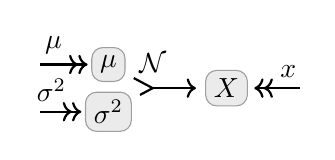
\begin{tikzpicture}[center base]
            \node[dpad0](X) at (0,0){$X$};
            % \node[dpad
            \draw[arr2, <<-] (X) to node[above,pos=0.7]{$x$} ++(1.0,0);
            % \draw[arr2, <-] (X) to node[above]{$\mathcal N(X|\mu,\sigma^2)$} ++(-1.7,0);
            \node[dpad0](m) at (-1.5, 0.3) {$\mu$};
            \node[dpad0](s2) at (-1.5, -0.3) {$\sigma^2$};
            \mergearr{m}{s2}{X};
            \node[above=2pt of center-ms2X](N){$\mathcal N$};
            \draw[arr1, <<-] (m) to node[above, pos=0.7]{$\mu$} +(-0.9,0);
            \draw[arr1, <<-] (s2) to node[above, pos=0.7]{$\sigma^2$} +(-0.9,0);
        \end{tikzpicture}}.
    \]

    The fisher information for a normal distribution is given by
    \[
    \mathcal I(\mu, \sigma) =
    % \begin{bmatrix}
    %     \Ex_{\mathcal N(X|\mu,\sigma^2}[ \frac{\partial mathcal N(X|\mu,\sigma^2}{\partial \mu}) ]
    % \end{bmatrix}
    % =
    \begin{bmatrix}
        \frac1{\sigma^2} & 0 \\
        0 & \frac{1}{2 \sigma^4}
    \end{bmatrix}
    \]



    The natural gradient update rule is given by
    \[
        F'_{x}(\mu, \sigma^2) = - \hat\nabla_{\mu, \sigma^2} \mathcal L(x,\mu,\sigma^2) = \mathcal I(\mu, \sigma^2)^{-1}
        \begin{bmatrix}
            \frac{x-\mu}{\sigma} \\[1ex] \frac {-\sigma^2 + (x-\mu)^2}{2 \sigma^4}
        \end{bmatrix}
        =
        \begin{bmatrix}
            x-\mu \\ (x-\mu)^2 - \sigma^2
        \end{bmatrix}
    \]

    Note that:
    \begin{itemize}
        \item  $\Ex_{x \sim \nu} [ F'_x(\mu,\sigma^2) ] = \mat 0$ if and only if $\nu$ has mean $\mu$ and variance $\sigma^2$.
        % We can interpret this in two ways:
        % This means that if observations are drawn from a fixed distribution $\nu(X)$,
        Moreover, this point is the unique global attractor.
        This means that, 
        \begin{enumerate}
            \item If observations are drawn from a fixed distribution $\nu(X)$, and we repeatedly use $F$ to update $\theta = (\nu, \sigma)$ with small confidence $\epsilon$,
            then $\mu$ will approach the mean $\Ex_{\nu}[X]$ of $\nu$
            and $\sigma^2$ will approach the variance $\Ex_{\nu}[X^2] - \Ex_{\nu}[X]^2$.             
            % If we make f observations are drawn from a fixed distribution $\nu(X)$,
            % If we update our belief parameters $\theta = (\mu, \sigma)$ according to $F$ with  
            
            \item If we perform a single high-confidence update on the extended observation $\varphi \propto \nu$, in which each $x$ has relative confidence $\nu(x)$, the result will be a Gaussian with the mean and variance of $\nu$, i.e.,
            \[ 
                \forall \theta.\quad
                \lim_{c \to \infty} \Pr\nolimits_{F_{\nu}^c(\theta)} = \mathcal N(\Ex\nolimits_{\nu}[X], {\mathrm{Var}}_{\nu}[X])
            \]
        \end{enumerate}
        In this sense, relative confidence acts like probability.
        % So, 
        
        \item 
        If we update with the observation $x = \mu$ of our estimate with confidence $c$,
        the mean is unchanged, and our estimate of the variance becomes the harmonic mean of our previous variance $\sigma_0^2$ and the inverse confidence $\frac1c$.
        That is, 
        \[
            F^c_\mu(\mu, \sigma_0^2) = 
            \left(\mu, \frac{1}{c + \frac{1}{\sigma_0^2}} \right).
        \]
        In particular, if $\sigma_0^2$ is very large, so that our initial beliefs say very little, updating with confidence $c$ results in variance $\frac1t$.
        In this sense, the magnitude of confidence acts as the inverse of variance.
    \end{itemize}
\end{examplex}


%

\section{Examples}
\subsection{Assorted}


\subsection{Relaxations of Bayes Rule (Updating By Conditioning)}
Fix some measurable space $\X = (X, \mathcal A)$ of possible outcomes, and consider an update rule for probability distributions $\Theta := \Delta\X$
on measurable events $\Phi = \mathcal A$.

The function
\[
    \mathrm{Bayes}^\beta_A(\mu) := \begin{cases}
            \mu \mid A &  \text{if }\beta > 0 \\
            \mu & \text{if } \beta = 0 \\
            \mu \mid \bar A &  \text{if } \beta < 0
        \end{cases}
\]
satisfies \cref{ax:zero,ax:additivity}, so it is an update rule.  But it is not differentiable in $\beta$ (it doesn't satisfy \cref{ax:diffble}).
% owever, it can be written as a limit of one that does:
% However, this behavior does arise as the limit of large $\beta$ for a differentiable update rule:
However, this behavior does arise as the limit of large-magnitude $\beta$ for a differentiable update rule. Consider the update rule
\begin{align*}
    F^\beta_A (\mu) &:\propto \mu \exp(\beta \mathbbm1[A]) \\
    F^\beta_A (\mu)(B) &:=
        % \mu(B) \exp(\beta \mathbbm1[A \cap B])
        \frac{1}{\Ex_{\mu}[e^{\beta\mathbbm1[A]}]}\int_{X}  \mathbbm1[B] \exp(\beta \mathbbm1[A]) \mathrm d\mu \\
        &=
        \frac{\mu(B\cap A)e^{\beta} + \mu(B \cap \bar A) }
        % {\mu(A)e^{\beta} + (1 - \mu(A))}
        {\mu(A)e^{\beta} + \mu(\bar A)}.
        % \int_{X}  \mathbbm1[B] \exp(\beta \mathbbm1[A]) \mathrm d\mu
\end{align*}

% It is easy to check that $F$ satisfies
% \cref{ax:zero,ax:additivity,ax:certainty,ax:symmetry,ax:commute,ax:diffble,ax:invert}.
% In addition to being a flow, this update rule
Note that
\begin{align*}
\lim_{\beta\to\infty} F^\beta_A(\mu) &= B \mapsto \frac{\mu(B \cap A)}{\mu(A)}
   = \mu \mid A; \\
 F^0_A(\mu) &= B \mapsto \mu(B); \qquad\text{and}\\
\lim_{\beta\to-\infty} F^\beta_A(\mu) &= B \mapsto \frac{\mu(B \cap \bar A)}{\mu(\bar A)}
      = \mu \mid \bar A.
\end{align*}
Thus, $\mathrm{Bayes} = \lim_{k \to \infty} F^{k}$, where $F^k$ is the update rule given by rescaling, as in \cref{prop:rescale}.



\begin{wip}
Is this the only such relaxation of Bayes Rule?

Suppose $F$ is another such relaxation, satisfying \cref{ax:zero,ax:additivity,ax:certainty,ax:symmetry,ax:commute,ax:diffble,ax:invert}.

\begin{prop}
    $F$ is unique up to curve reparameterization.
\end{prop}

By differentiability (\cref{ax:diffble}) and \cref{thm:vecrep}, we know that $F$ is generated by vector field $F' : \mathcal A \times \Delta\X \to \Delta\X$.
We start by investigating the action on singletons.
\[
    F'_{\{x\}}(\mu)
\]

Assuming that the vector field is conservative,

\begin{conj}
    $F$ is the unique update rule, up to multiplicative scaling, satisfying
    \cref{ax:zero,ax:additivity,ax:certainty,ax:symmetry,ax:commute,ax:diffble,ax:invert}
\end{conj}
\end{wip}


\subsection{Case Study: Jeffrey's Rule}
\subsection{Mixture of Experts}

\subsection{Weight of Evidence}
\subsection{Loss Functions}
\subsection{Bolzman Rationality}

\begin{examplex}{}{}
    Consider a neural network whose output is a c
\end{examplex}

% Loss Functions
% Total \# of Updates
\section{Confidence in PDGs}
\subsection{Quantitative PDGs}

\subsubsection{Updating Second-Order Distributions with PDGs}
Let $\mat X$ be a set of variables, where each variable $X \in \mat X$ can take possible values in the set $\V(X)$, and let $\V(\mat X)$ be the set of possible joint settings of all variables in $\mat X$.

\begin{align*}
    \Theta &:=
        \Big\{
        \text{Second-order probabilities}~ \Pr \in \Delta^2 \V(X)
        \Big\} \\
    % \Phi &:= \Big\{ \text{PDGs}~ \dg M
    %     \text{ with variables } \N^{\dg M} = \mat X \Big\}
    \Phi &:= \Big\{ \text{cpds}~ p(Y|X)
        % \text{ where }  X, Y \in \mat X \Big\}
        \text{ where }  X, Y \subset \mat X \Big\}
        %%% TODO: What about hypergraph fs non-hypergraph distinction?
\end{align*}

Now, consider the Bolzmann update rule
% Given a PDG $\dg M$, let $\X := \Delta\V(\dg M) = \Delta(\prod_{X\in\N}\V(X))$. For each edge we have
\[
    F_L^{\beta}(\Pr) (\mu) \propto \Pr(\mu) \exp(-\beta \kldiv\mu \bp)
\]

% Note, that the free extension of $\Phi$ is
Note, that the free extension of $\Phi$ is isomorphic to the set of ``purely quantitative'' PDGs, i.e., those with $\balpha = \mat 0$, over the variables $\mat X$:
$$
    % \bar\Phi = \{ \text{PDGs}~\dg M \text{ with variables } \N^{\dg M} = \mat X \Big\}
    \bar\Phi = \Big\{ \text{PDGs}~\dg M = (\mat X, \Ed, \bP[], \mat0, \bbeta) \Big\}
$$
and it is easily verified that update rule from before extends to
\[
    F_{\dg M}^k(\Pr)(\mu) \propto \Pr(\mu) \exp(- k \bbr{\dg M}_0(\mu))
\]
Note that
\begin{align*}
    \lim_{k \to \infty} F_{\dg M}^k(\Pr)(\mu) &\propto
        % \mathbbm1[\mu \in {\displaystyle\SD{\dg M}}]
        \Pr(\mu) \mathbbm1[\mu \in {\bbr{\dg M}^*_0}] \\
        &= \Pr \,|\, \bbr{\dg M}^*_0 \\
        &= \Pr \,|\, \SD{\dg M} \text{~if $\dg M$ is consistent.}
        % &= \mathrm{Unif}_{\{\!\!\{{\dg M}\}\!\!\}} \text{~if $\dg M$ is consistent.}
\end{align*}

That is to say, applying the update with observation $\dg M$ and infinite certainty is like conditioning the higher-order distribution $\Pr$ on those distributions $\mu$ consistent with $\dg M$.
% On the other hand,
Now we turn to the opposite extreme, when confidence is low. When $k=0$, clearly $F^k_\dg M(\Pr) = \Pr$, so $F$ satisfies \cref{ax:zero}. And in the limit, as $\gamma \to 0$,
\begin{align*}
    \lim_{k \to 0} F_{\dg M}^k(\Pr)(\mu) &= \Pr \,|\, \{ \Inc_{\dg M}(\mu) < \infty \} \\
        &= \Pr \,|\, \{\mu : \forall L.~\mu(Y|X) \ll \bp \}.
        % \quad\Big(\text{i.e., if $\mu$ is absolutely continuous with respect to $\bp$}
        % \Big)
\end{align*}

So $F$ can only be continuous at $k=0$ for $\Pr$ (and hence can only satisfy \cref{ax:diffble}) if, for all edges $L \in \Ed$, we have that $\Pr(\mu(Y|X) \ll \bp) = 1$.
So one easy way to ensure differentiability for all update rules is to require strictly positive probabilities in theprobabilities in the cpds.



\subsubsection{Updating Distributions with PDGs and Incompatibility}
% \def\tauur{\mathtt T}
% \def\tauur{\mathtt{GD}}
% \def\tauur{\tau}
\def\tauur{\mathtt{CPD\_UR}}

\begin{align*}
    \Theta &:=
        \Big\{
        \text{Probabilities}~ \mu \in \Delta \V(\mat X)
        \Big\} \\
    \Phi &:= \Big\{ \text{cpds}~ p(Y|X)
        % \text{ where }  X, Y \in \mat X \Big\}
        \text{ where }  X, Y \subset \mat X \Big\}
\end{align*}

Given a cpd $p(Y|X)$ with $X,Y \subset \mat X$,
define an update rule on joint distributions $\mu$ by
\begin{align*}
    % (\tau_{p(Y|X)}^\beta \mu) (\mat X) \propto
    %     \mu(X) \left(\frac{p(Y|X)}{\mu(Y|X)}\right)^{1 - e^{-\beta}} \mu(\mat X\setminus\{X,Y\}\mid X,Y)
    \Big(\tauur_{p(Y|X)}^\beta \mu\Big) (\mat X) &\propto
        \mu(\mat X) \left(\frac{p(Y|X)}{\mu(Y|X)}\right)^{1 - e^{-\beta}}
\end{align*}
    %
    % \\
    % &= \mu(X) p(Y|X)^{e^{-\beta}} \mu(Y|X)^{1-e^{-\beta}}  \mu(\mat X\setminus\{X,Y\}\mid X,Y)
%     &= \mu(X)\; p(Y|X)^{\epsilon} \mu(Y|X)^{1-\epsilon}  \mu(Z\mid X,Y)
% \end{align*}
Writing this in a
where $\epsilon := 1-e^{-\beta}$ and $Z := \mat X \setminus \{X,Y\}$.

\begin{prop}
    $\tauur_{p(Y|X)}$
\end{prop}

\begin{prop}
    The vector field of $\ext\tauur$ is the natural gradient of $\Inc_{\dg M}$, i.e.,
    $
        % \tau'_{\dg M}(\mu) = - \hat \nabla_\mu \bbr{\dg M}_0(\mu),
        \ext\tauur'_{\dg M} = - \hat \nabla \Inc_{\dg M},
    $
    so $\tauur$ is the update rule on joint distributions which reduces incompatibility by locally moving in the direction of steepest descent.
\end{prop}

\begin{prop}
    % \begin{enumerate}
        % \item \relax \texttt{\color{red}[CONJECTURE]}~
        % $\displaystyle
        %     \tauur_{\dg M}^{\{\nf1\gamma\}}(\mathrm{Unif}) \in \bbr{\dg M}_{\gamma}^*
        % $
        %
        % \item
        Updating $\dg M$ with absolute certainty computes the information projection onto the convex set of distributions consistent $\dg M$ i.e.,
        $$\displaystyle
            \tauur_{\dg M}^\infty(\mu) = \argmin_{\mu' \in \SD*{\dg M}} \kldiv{\mu'}{\mu}
        $$

    % \end{enumerate}
\end{prop}


\subsubsection{Updating PDGs with PDGs, via inconsistency reduction}
\begin{align*}
    \Theta :=
        \Big\{
        \text{PDGs}
        \Big\}; \qquad
    \Phi := \Big\{ \text{PDGs} \Big\}
\end{align*}

% Of course, we often think
We now consider the more general setting, in which both the observations $\Phi$ and the belief states $\Theta$ are 
Here's an update rule that simply adds the new data to a PDG.
\[
    F^{\beta}_{p(Y|X)}(\dg M) = \dg M ~+~
        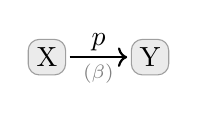
\begin{tikzpicture}[center base]
            \node[dpad0](X) {X};
            \node[dpad0,right=0.8 of X](Y) {Y};
            \draw[arr1](X) to
                node[above,inner sep=2pt]{$p$}
                node[below,inner sep=2pt]{${\scriptstyle\color{gray}(\beta)}$} (Y);
        \end{tikzpicture}
\]

It's extension is the update rule that incorporates data of the new PDG to the old one, where all confidences in the new PDG are scaled by $k$.
\[
    % F^{\beta}_{\dg M'}(\dg M) = \dg M ~+~ \beta\,\dg M'
    \bar F^{k}_{\dg M'}(\dg M) = \dg M ~+~ k\,\dg M'
\]

% There are actually several natural 
The colletion of all PDGs, even on a finite set of finite variables, does not naturally form a manifold of fixed finite dimension. 
But if we restrict our attention to PDGs with a certain fixed structure, then it does. 
But, per \parencite{richardson2022loss}, we already have a natural choice of a loss $\mathcal L = \aar{-} : \mathrm{PDG} \times \mathrm{PDG} \to \mathbb R$: the inconsistency of the joint PDG.

Still, there is more than one reasonable way to perform updates: we can adjust the internal confidences $\bbeta$ of our PDG, or its cpds $\mat p$. 
% The first is closer to a mixture of experts approach, and the latter 

\[
    \bar G'_{\dg M'}(\dg M) = - \hat\nabla_{\mat p} \aar{\dg M + \dg M'}
\]

\begin{openQ}
    How do $\bar F$ and $\bar G$ relate to one another?
\end{openQ}

\begin{conj}
    $\tauur$ should be a special case. 
\end{conj}

\subsubsection{}
\begin{align*}
    \Theta :=
        \Big\{
        \text{PDGs over variables } \mat X
        \Big\}; \qquad
    % \Phi := \Big\{
    %     \text{Probabilities}~ \mu \in \Delta \V(\mat X)
    %     \Big\}
    \Phi := \Big\{
        \text{Probabilities}~ \mu \in \Delta \V(\mat X)
        \Big\}
\end{align*}



\end{document}
